% SPDX-License-Identifier: Apache-2.0
% Generated by maintenance/build_manual.py from docs/manual-content.json.
% Compile here with: latexmk -pdf -interaction=nonstopmode -halt-on-error main.tex
% For project updates edit the shared JSON; this TeX export can also be compiled/edited independently.
\documentclass[a4paper,landscape,10pt]{article}
\usepackage{manual}
\newcommand{\manualversion}{0.2.1.dev0}
\newcommand{\manualdate}{2026-10-27}
\hypersetup{pdftitle={texstage user manual},pdfauthor={texstage project}}
\begin{document}

% texstage user manual
\pdfbookmark[0]{texstage user manual}{cover}
{\fontsize{28}{34}\selectfont\bfseries texstage user manual\par}
\vspace{2mm}
{\Large\color{manualPurple} Presenter and participant guide\par}
\vspace{3mm}
A practical guide to presenting Beamer decks, running live quizzes and participating from a phone.\par

For presenters and participants. Includes a first-session walkthrough, illustrated controls, answer formats, exports and a participant quick reference.\par

\medskip
\begin{minipage}[t]{0.73\linewidth}
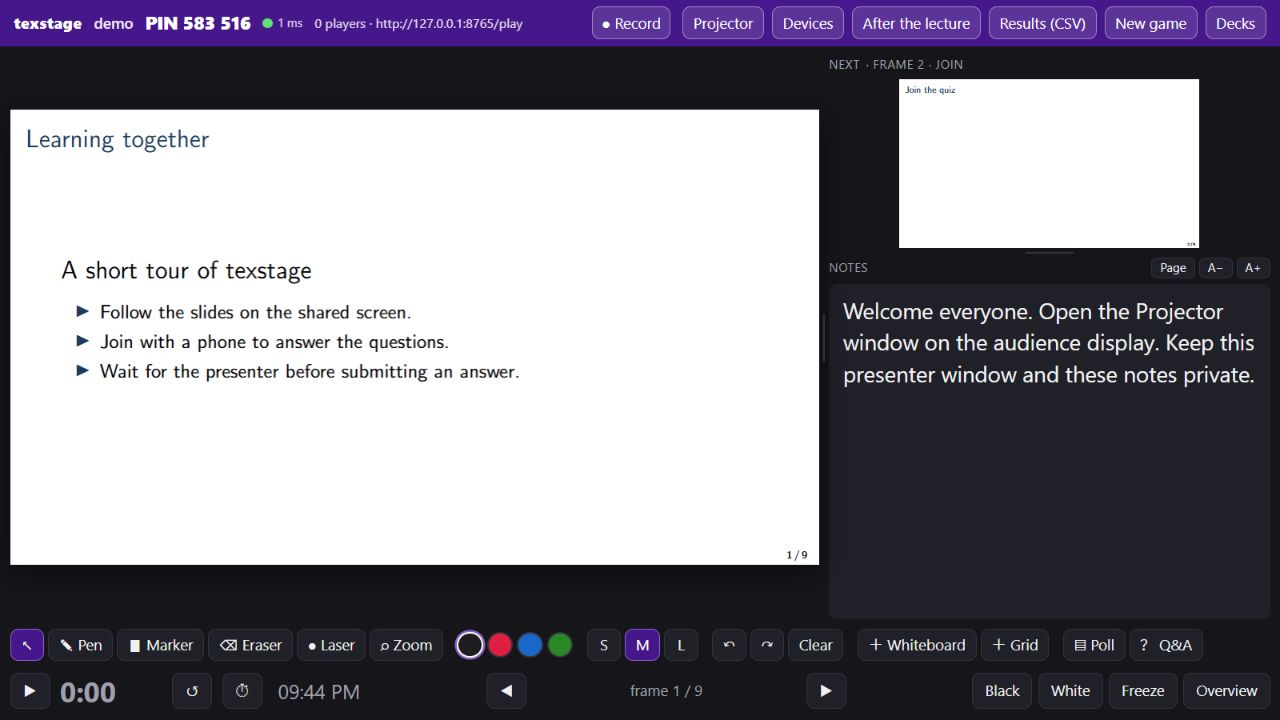
\includegraphics[width=\linewidth]{../images/manual/02-presenter-workspace.jpg}\par
{\manualcaption The private presenter workspace.\par}
\end{minipage}\hfill%
\begin{minipage}[t]{0.19\linewidth}
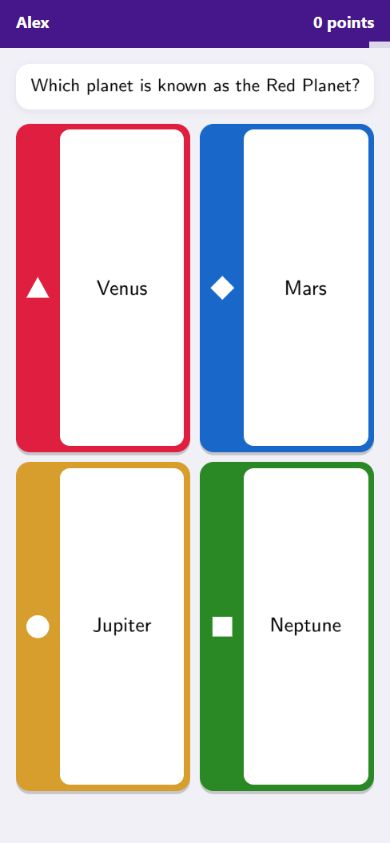
\includegraphics[height=99mm]{../images/manual/08-phone-single-choice.jpg}\par
{\manualcaption A participant answers in the browser.\par}
\end{minipage}\par\medskip
{\small\color{manualMuted} Version 0.2.1.dev0 - unpublished development candidate. Screenshots use a synthetic session and a mobile-sized browser viewport; they are not photographs of a physical phone.\par}
\clearpage
{\setlength{\parskip}{0pt}\tableofcontents}

% Start your first session
\manualsection{Start your first session}
Use the new texstage checkout and a fresh Python 3.12+ environment. Deck builds need pdflatex and Beamer from TeX Live or MiKTeX. The source checkout contains the examples and dependency locks used below. The candidate is not assumed to be available on PyPI.\par

\manualsubheading{1  Create and activate an environment}
\begin{Verbatim}
python -m venv .venv
# Windows PowerShell
.\.venv\Scripts\Activate.ps1
# Linux or macOS
# . .venv/bin/activate
\end{Verbatim}

\manualsubheading{2  Install the locked dependencies and this checkout}
\begin{Verbatim}
python -m pip install --require-hashes --only-binary=:all: -r requirements/runtime.txt
python -m pip install --require-hashes --only-binary=:all: -r requirements/build.txt
python -m pip install --no-deps --no-build-isolation .
\end{Verbatim}

\manualsubheading{3  Preview and present the example}
\begin{Verbatim}
texstage pdf --present examples/manual/demo.tex
texstage present examples/manual/demo.tex --data .manual-data --port 8765 --no-tunnel
\end{Verbatim}

Use an unused port for rehearsal (8765 in this example). The present command builds a missing or out-of-date deck, starts a local server if needed, and opens the browser presenter. Use its printed server address. If a server is already running on that port, present reuses it; choose another port to keep the demo separate. The manual uses long 240-second rounds for rehearsal.\par

For environment activation, missing TeX packages and wheel-only installation, see \href{../installation.md}{installation.md}. For an already configured environment, start at step 3. Keep existing course environments and tools pins unchanged during rehearsal.\par


% Choose a deck
\manualsection{Choose a deck}
\begin{minipage}[t]{0.665\linewidth}\vspace{0pt}
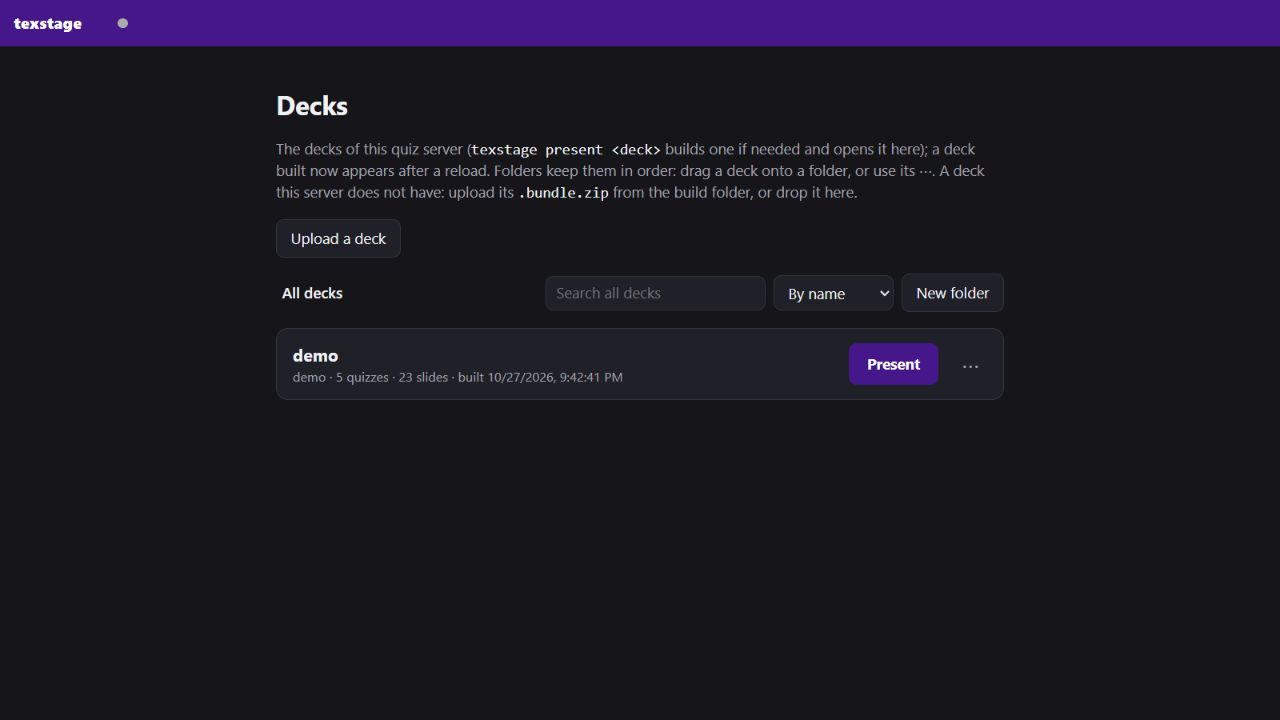
\includegraphics[width=\linewidth]{../images/manual/01-deck-library.jpg}\par
{\manualcaption Deck library. Present opens the private presenter workspace; the three-dot menu contains deck actions.\par}
\end{minipage}\hfill%
\begin{minipage}[t]{0.305\linewidth}\vspace{0pt}
\manualsubheading{Open the library}
The presenter is at \texttt{/stage} on your quiz server. On the server laptop it normally obtains the local presenter key automatically. A remote presenter uses an authorized key or a paired device.\par

\begin{itemize}
\item Choose \textbf{Present} on the deck you want to use.
\item Use search to find a deck across folders. Choose \textbf{By name} or \textbf{Newest first} to change the order.
\item Use \textbf{New folder} and the deck actions menu to organize your library.
\item Use \textbf{Upload a deck} for a \texttt{.bundle.zip} created by texstage build. Upload the bundle, not an arbitrary PDF.
\end{itemize}

A deck built while the library is open appears after a reload. A browser presentation requires a build containing the stage PDF; rebuild without \texttt{--no-stage} if it is missing.\par

\end{minipage}

% Know your presenter workspace
\manualsection{Know your presenter workspace}
\begin{minipage}[t]{0.665\linewidth}\vspace{0pt}
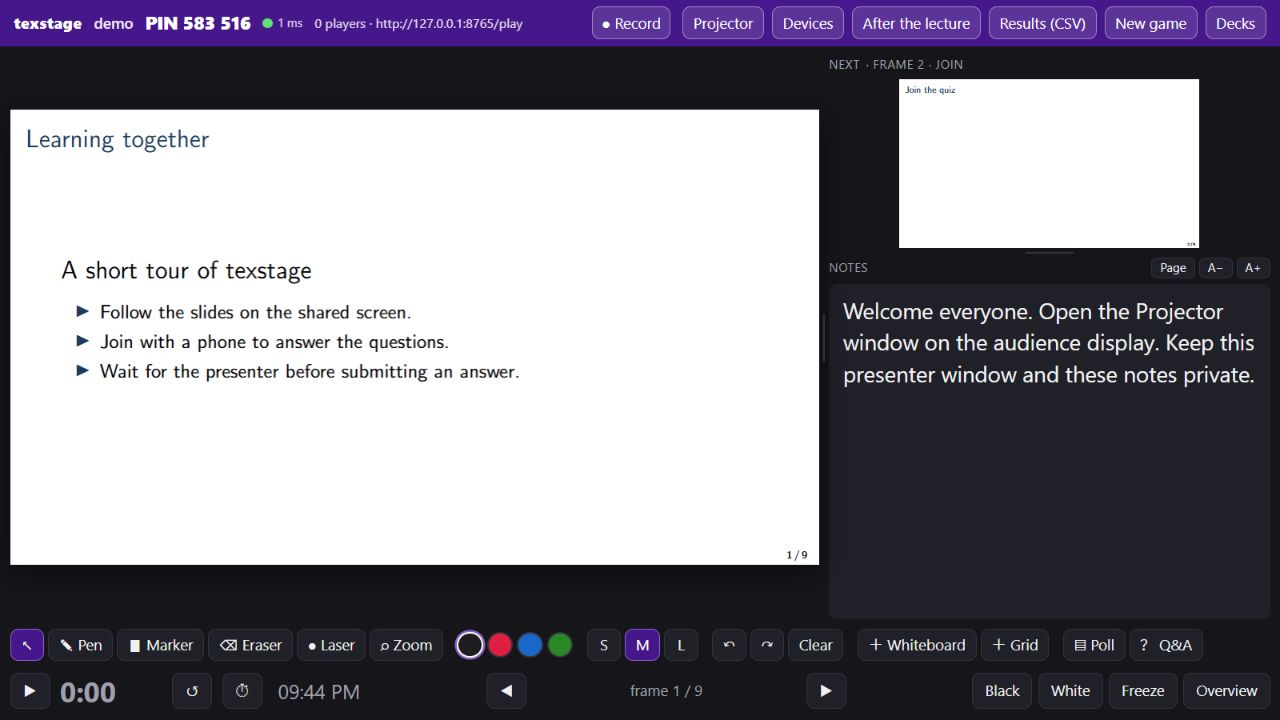
\includegraphics[width=\linewidth]{../images/manual/02-presenter-workspace.jpg}\par
{\manualcaption Presenter workspace with text notes. Next previews the join slide. The elapsed lecture timer is separate from a quiz countdown.\par}
\end{minipage}\hfill%
\begin{minipage}[t]{0.305\linewidth}\vspace{0pt}
\begin{itemize}
\item \textbf{Current slide, left:} the step being presented, including live quiz content.
\item \textbf{Next, upper right:} a preview of the next step. It may show the correct answer before the audience sees it.
\item \textbf{Notes, lower right:} switch between rendered \textbf{Page} and \textbf{Text} views. Use \textbf{A- / A+} for text size.
\item \textbf{Top bar:} session PIN, connection indicator, latency, player count and join address. Projector, exports and session controls are here.
\item \textbf{Bottom bar:} annotation tools, slide navigation, elapsed timer, display controls and Overview.
\end{itemize}

Show the \textbf{Projector} window to the audience. Keep this presenter window private: its notes, previews and controls are for you. Drag the dividers to adjust the slide and notes areas; double-click a divider to restore its default position.\par

\end{minipage}

% Connect the audience
\manualsection{Connect the audience}
{\centering\begin{minipage}{190mm}
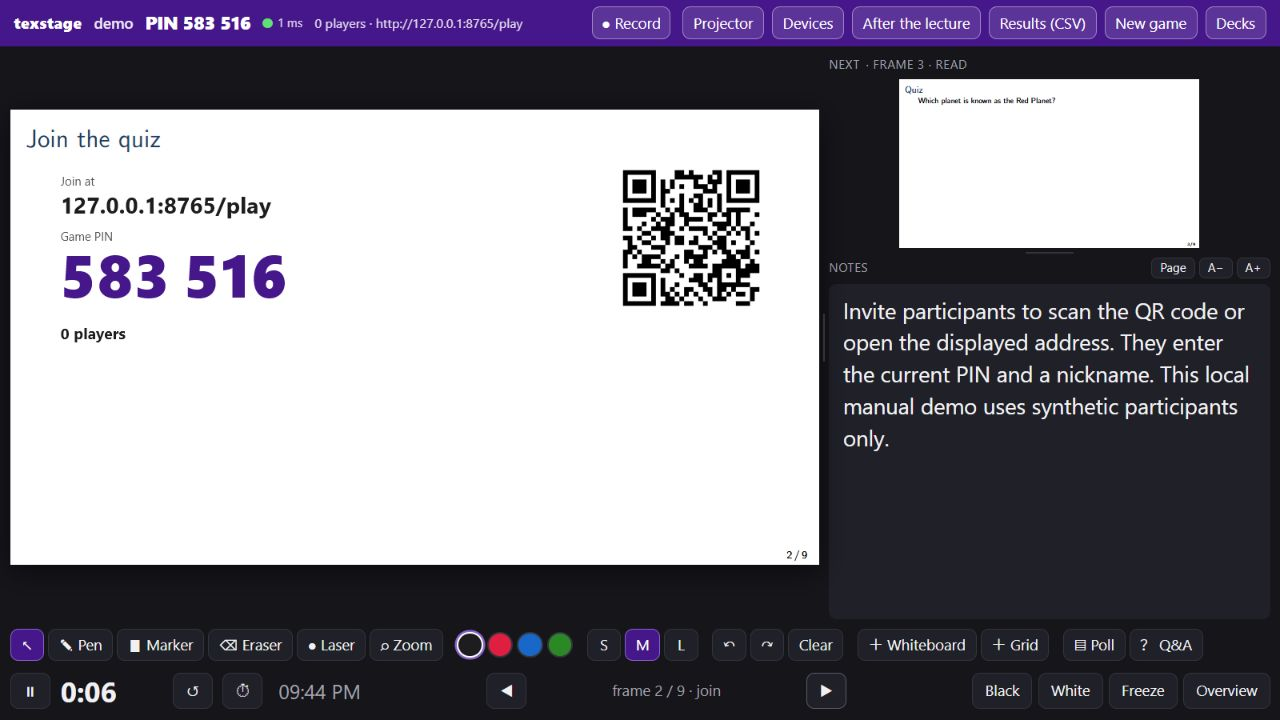
\includegraphics[width=\linewidth]{../images/manual/03-presenter-join.jpg}\par
{\manualcaption The join slide shows the session address, PIN, QR code and player count. The PIN shown here is only an example.\par}
\end{minipage}\par}\medskip
\begin{itemize}
\item Choose \textbf{Projector}, move that window onto the audience display, and use an extended desktop. If a pop-up is blocked, allow the projector window for this server. The projector can enter full screen when clicked; F is the presenter freeze shortcut, not its full-screen command.
\item Advance to the join slide. Participants scan its QR code or open its address, enter the current PIN and choose a nickname.
\item Test the join address on a real phone before the session. The screenshots use 127.0.0.1 for a local demonstration; on a phone that address points to the phone itself. Use the reachable address printed by your actual server.
\end{itemize}


% Join and wait on your phone
\manualsection{Join and wait on your phone}
{\centering
\begin{minipage}[t]{65mm}\centering
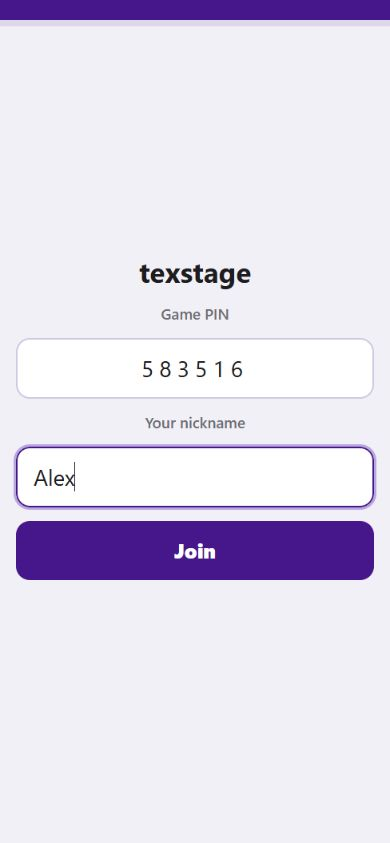
\includegraphics[height=108mm]{../images/manual/04-phone-join.jpg}\par
{\manualcaption Enter the current PIN and a nickname.\par}
\end{minipage}%
\hspace{5mm}%
\begin{minipage}[t]{65mm}\centering
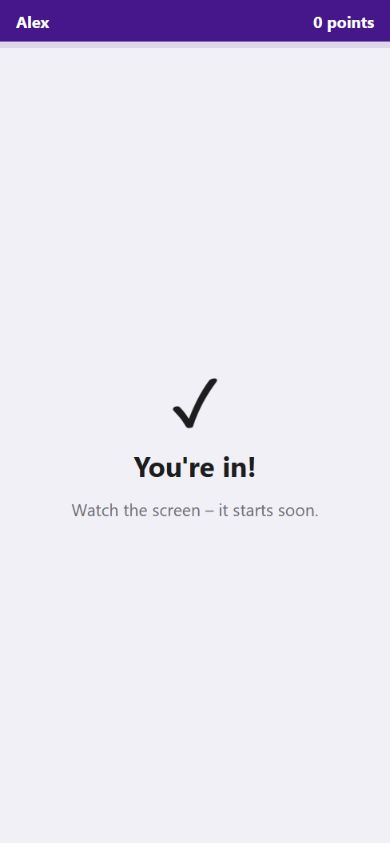
\includegraphics[height=108mm]{../images/manual/05-phone-lobby.jpg}\par
{\manualcaption Wait for the presenter after joining.\par}
\end{minipage}%
\hspace{5mm}%
\begin{minipage}[t]{65mm}\centering
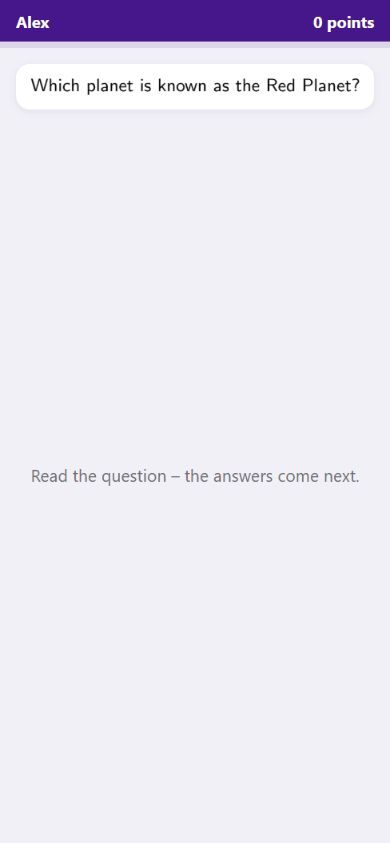
\includegraphics[height=108mm]{../images/manual/06-phone-reading.jpg}\par
{\manualcaption Read first; the answers open on the next step.\par}
\end{minipage}%
\par}\medskip
No app installation is needed. Open the session address in a browser, enter the PIN shown in the room and a nickname, then tap \textbf{Join}. A QR code may prefill the PIN. \textbf{You're in!} confirms that joining succeeded.\par

When the question appears, read it first. The reading screen deliberately has no answer buttons. Wait for the presenter to advance again. Keep this browser tab open throughout the session.\par


% Run a timed question
\manualsection{Run a timed question}
\begin{minipage}[t]{0.665\linewidth}\vspace{0pt}
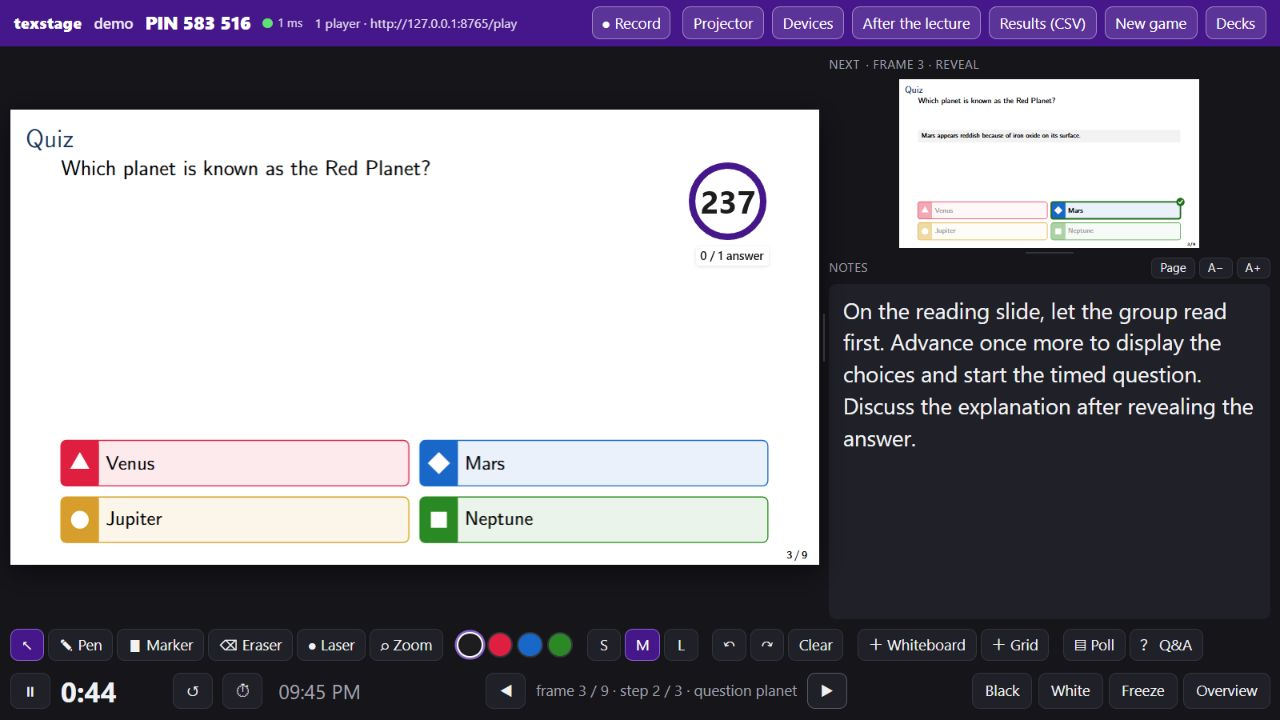
\includegraphics[width=\linewidth]{../images/manual/07-presenter-question.jpg}\par
{\manualcaption A question is open, with its countdown and answer counter. The private Next pane already previews the reveal.\par}
\end{minipage}\hfill%
\begin{minipage}[t]{0.305\linewidth}\vspace{0pt}
\begin{itemize}
\item \textbf{Read:} advance onto the reading step. The question appears on the shared screen and phones, without starting the round.
\item \textbf{Open:} advance once more. A three-second Get ready countdown precedes the answer timer.
\item \textbf{Control:} move the pointer over the live quiz to find \textbf{Pause}, \textbf{+10 s} and \textbf{Stop the question}. Pausing the quiz also pauses the answering interface on phones.
\item \textbf{Close:} the round can close when the time runs out, when all connected participants have answered, or when you stop it.
\item \textbf{Reveal:} advance to the reveal step or use \textbf{Show the answer} when offered. Discuss the explanation and results.
\end{itemize}

The answer counter is accepted answers / (accepted answers + connected players still waiting). A submitted answer remains counted if its phone disconnects. Unanswered offline participants drop out of the denominator until they reconnect.\par

\end{minipage}

% Submit an answer and read feedback
\manualsection{Submit an answer and read feedback}
{\centering
\begin{minipage}[t]{65mm}\centering
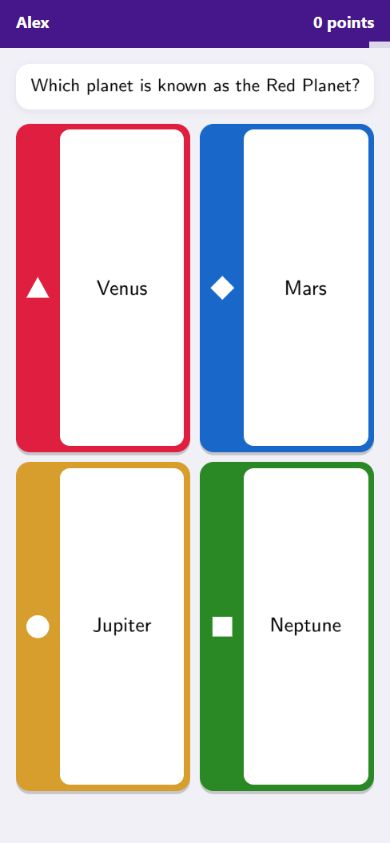
\includegraphics[height=108mm]{../images/manual/08-phone-single-choice.jpg}\par
{\manualcaption Tap one answer in a single-choice round.\par}
\end{minipage}%
\hspace{5mm}%
\begin{minipage}[t]{65mm}\centering
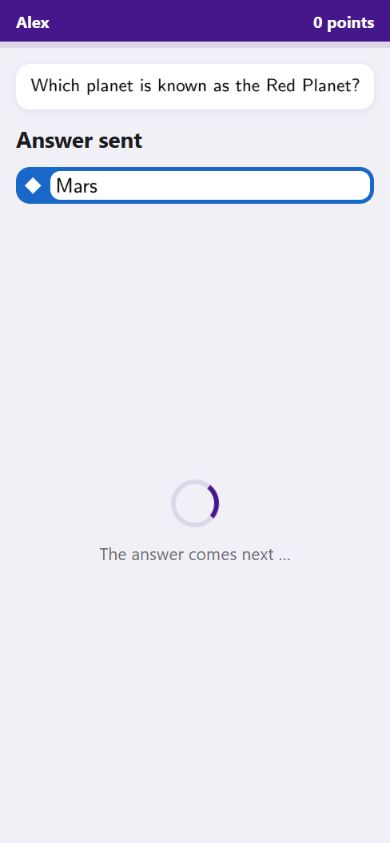
\includegraphics[height=108mm]{../images/manual/09-phone-answer-sent.jpg}\par
{\manualcaption The submitted answer is acknowledged.\par}
\end{minipage}%
\hspace{5mm}%
\begin{minipage}[t]{65mm}\centering
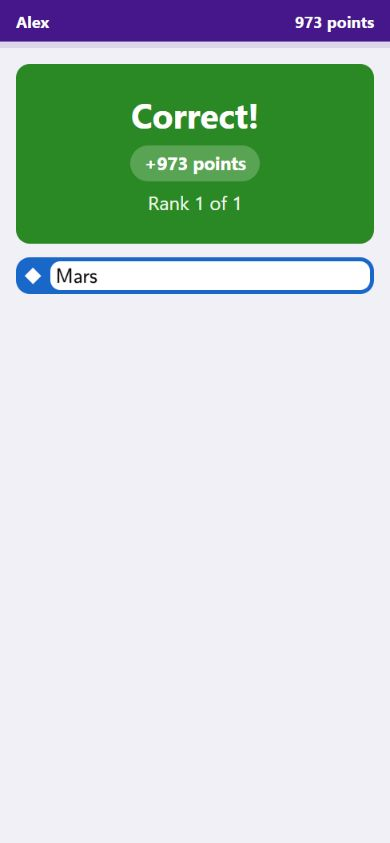
\includegraphics[height=108mm]{../images/manual/11-phone-feedback.jpg}\par
{\manualcaption Feedback appears after the presenter reveals it.\par}
\end{minipage}%
\par}\medskip
For a single-choice or true/false question, tap one answer to submit it immediately. For multiple selections and other input forms, use \textbf{Submit}. \textbf{Answer sent} confirms acceptance; wait for the reveal rather than tapping again.\par

After reveal, the phone shows the result, points and rank when scoring is enabled. Polls and practice rounds have different feedback. The score here is illustrative: timing, question settings and streaks can affect points.\par


% Reveal and discuss the result
\manualsection{Reveal and discuss the result}
{\centering\begin{minipage}{190mm}
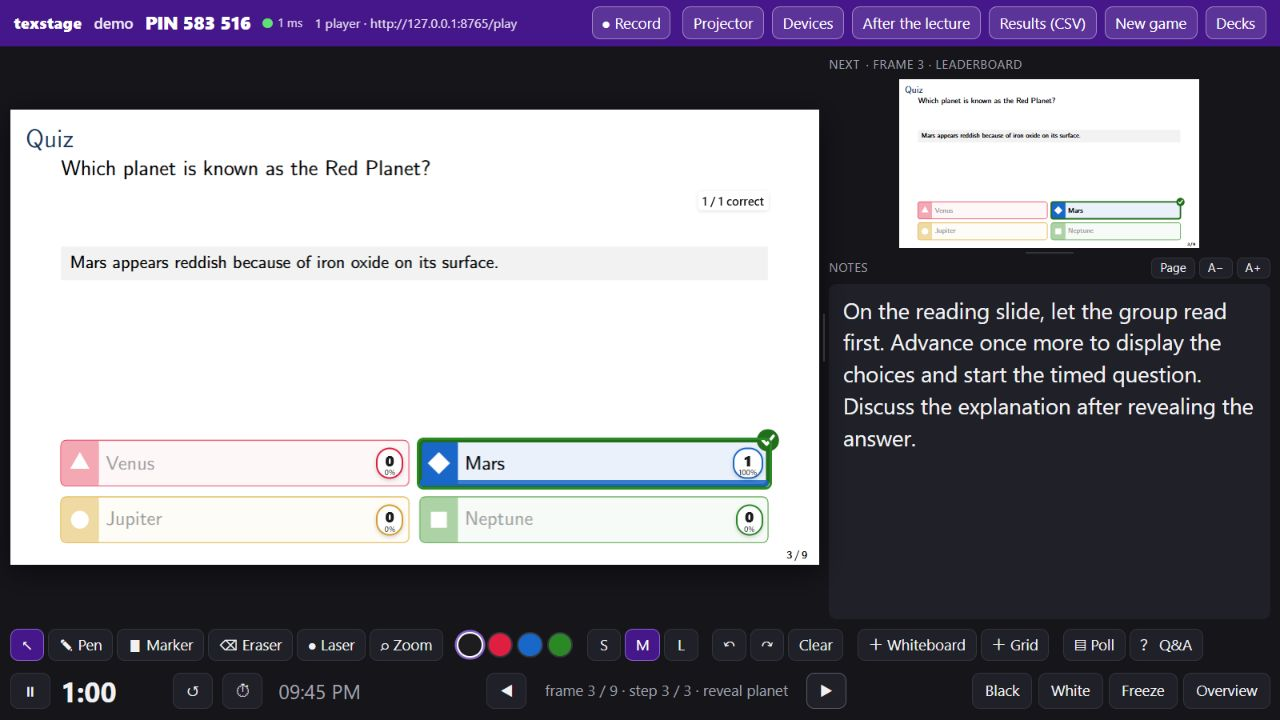
\includegraphics[width=\linewidth]{../images/manual/10-presenter-reveal.jpg}\par
{\manualcaption Reveal view for the planet question. The correct answer is marked and the authored explanation is visible.\par}
\end{minipage}\par}\medskip
\begin{itemize}
\item The reveal can show the correct choices, response counts and an explanation authored in the deck. Give the group time to discuss why an answer is correct.
\item Going backwards does not automatically restart a question. Its previous state and results are retained.
\item \textbf{Ask again (practice)} reruns the question without points and rewinds later questions so they can run anew. Use it deliberately: it also discards the affected later answers and points. Use \textbf{New game} for a fresh group and a new PIN.
\end{itemize}


% Use the different answer formats
\manualsection{Use the different answer formats}
{\centering
\begin{minipage}[t]{65mm}\centering
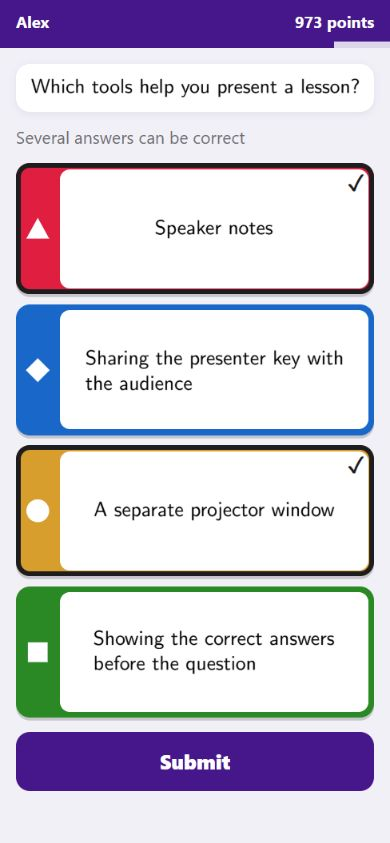
\includegraphics[height=108mm]{../images/manual/13-phone-multiple-choice.jpg}\par
{\manualcaption Multiple selections need an explicit Submit.\par}
\end{minipage}%
\hspace{5mm}%
\begin{minipage}[t]{65mm}\centering
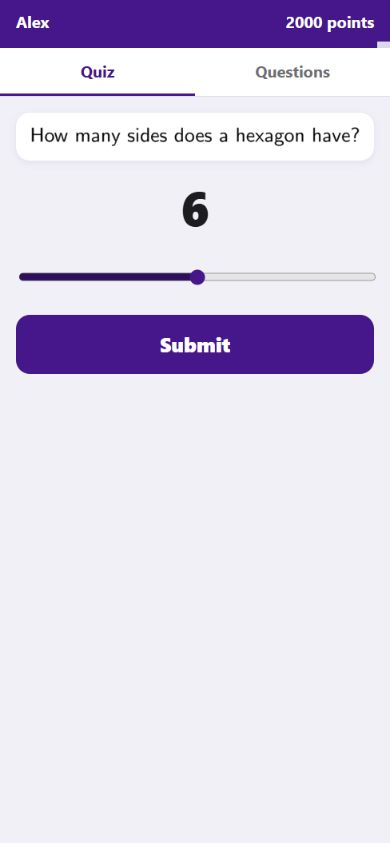
\includegraphics[height=108mm]{../images/manual/16-phone-numeric.jpg}\par
{\manualcaption Numeric input can be a bounded slider.\par}
\end{minipage}%
\hspace{5mm}%
\begin{minipage}[t]{65mm}\centering
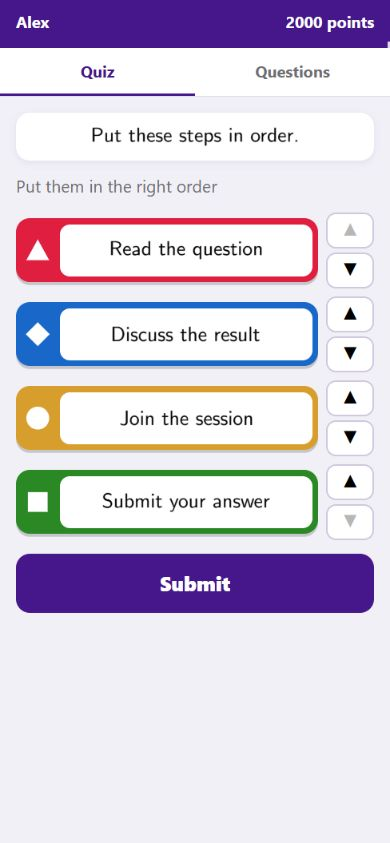
\includegraphics[height=108mm]{../images/manual/17-phone-ordering.jpg}\par
{\manualcaption Reorder the items using the up/down buttons.\par}
\end{minipage}%
\par}\medskip
For \textbf{multiple choice}, tap every intended answer and then \textbf{Submit}; selected answers have check marks. For \textbf{numeric} questions, set the slider or enter a number, check its units and submit. For \textbf{ordering}, use the up/down buttons to arrange the items before submitting.\par

Text and open-response questions provide a text field. Sketch questions provide a drawing pad with pen colors, Undo, Clear and Submit. A poll can use one or several choices and has no correct answer. Follow the instructions shown on that round.\par


% Navigate and control the shared display
\manualsection{Navigate and control the shared display}
\begin{minipage}[t]{0.665\linewidth}\vspace{0pt}
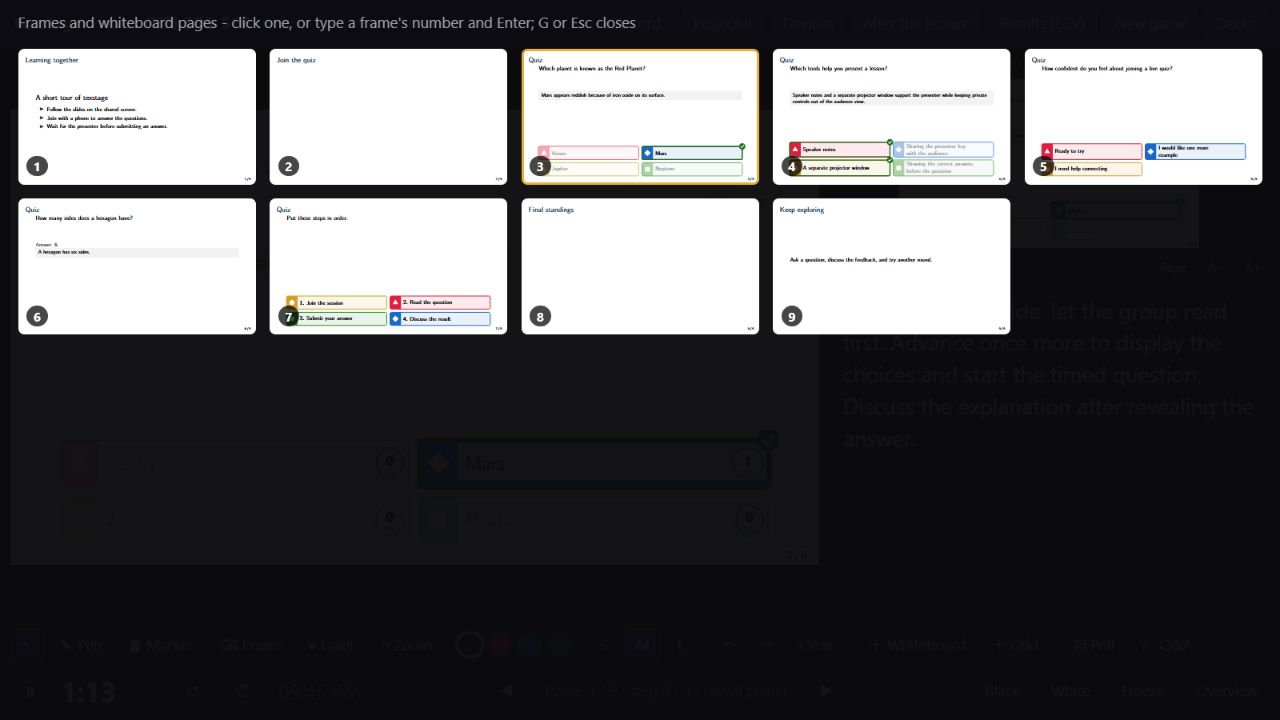
\includegraphics[width=\linewidth]{../images/manual/12-presenter-overview.jpg}\par
{\manualcaption Overview displays one thumbnail per frame and lets the presenter jump directly. Correct answers can be visible in these thumbnails.\par}
\end{minipage}\hfill%
\begin{minipage}[t]{0.305\linewidth}\vspace{0pt}
\manualsubheading{Move through the deck}
Use \textbf{Next / Previous}, the arrow keys, PageDown / PageUp, or a clicker. Space and Enter also advance. A frame can contain several steps: reading, answering and reveal are different steps of the same quiz frame.\par

Choose \textbf{Overview} or press \textbf{G} to jump to a frame. Type a frame number and press Enter to jump directly. Home and End go to the first and last steps. Esc closes the overview or leaves a selected tool.\par

\manualsubheading{Control what the room sees}
\begin{itemize}
\item \textbf{Black (B)} or \textbf{White (W)} temporarily covers the projector output.
\item \textbf{Freeze (F)} holds the projector while you navigate privately. Select it again to resume live display.
\item \textbf{T} controls the elapsed lecture timer. It does not pause a live quiz round.
\end{itemize}

Keep the overview private: its thumbnails may include reveal answers. Test your clicker and projector window before participants arrive.\par

\end{minipage}

% Ask and moderate audience questions
\manualsection{Ask and moderate audience questions}
\begin{minipage}[t]{49mm}\vspace{0pt}
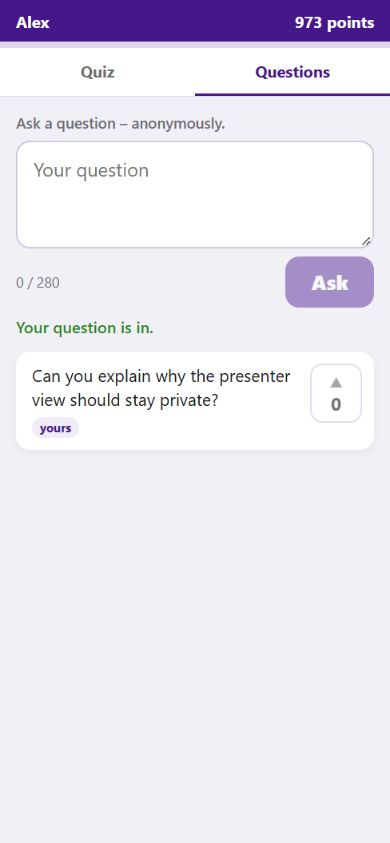
\includegraphics[width=49mm]{../images/manual/14-phone-questions.jpg}\par
{\manualcaption A participant submits a question from the Questions tab.\par}
\end{minipage}\hfill%
\begin{minipage}[t]{195mm}\vspace{0pt}
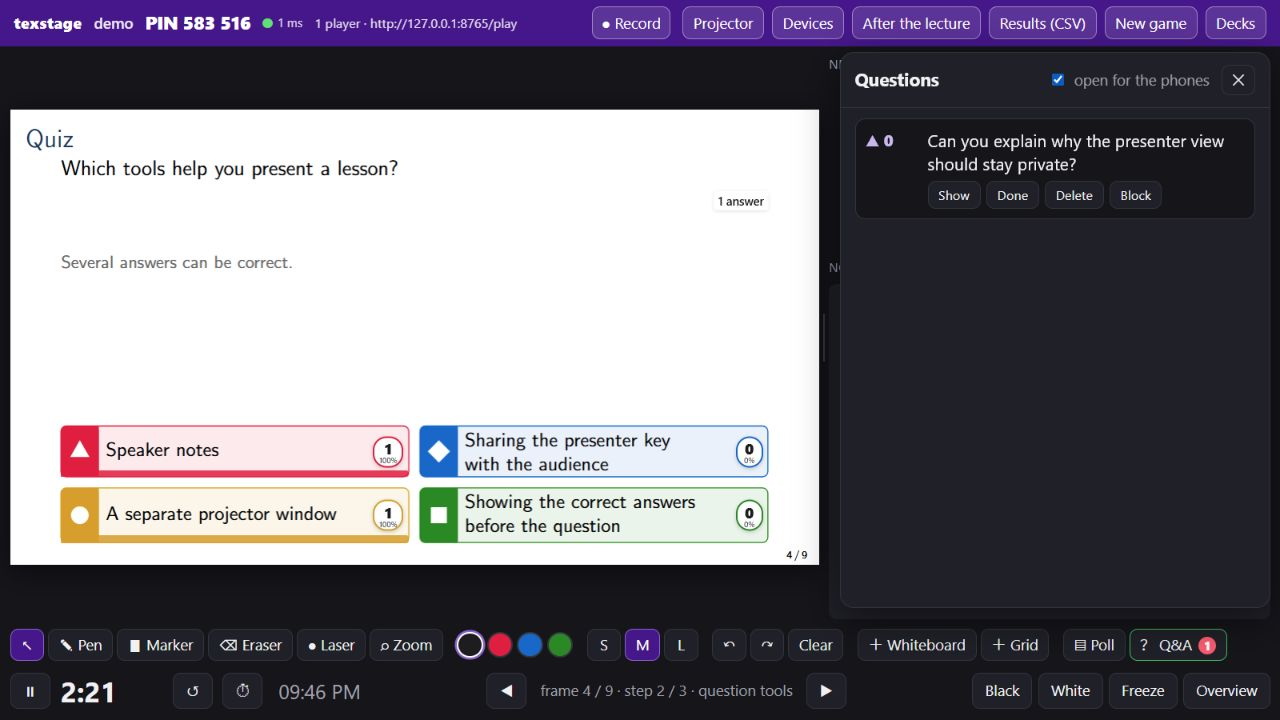
\includegraphics[width=\linewidth]{../images/manual/15-presenter-questions.jpg}\par
{\manualcaption The presenter chooses which question to show and when to mark it done.\par}
\end{minipage}\par\medskip
In the presenter, open \textbf{Q\&A} and enable \textbf{open for the phones}. Participants then get a \textbf{Questions} tab where they can submit a question and upvote another open question. Their own question cannot be upvoted by them.\par

Use \textbf{Show} to place a question on the projector, \textbf{Hide} to remove it from the screen, and \textbf{Done} when it has been addressed. Delete and Block are moderation actions. Closing the panel alone does not close submissions; turn off \textbf{open for the phones} when finished. Questions are displayed without the participant nickname.\par


% Use annotation and optional presenter tools
\manualsection{Use annotation and optional presenter tools}
{\small
\begin{tabular}{>{\raggedright\arraybackslash}p{\dimexpr0.200000\linewidth-2\tabcolsep\relax}>{\raggedright\arraybackslash}p{\dimexpr0.800000\linewidth-2\tabcolsep\relax}}
\rowcolor{manualPurple}
\color{white}\bfseries Tool & \color{white}\bfseries How to use it \\
Pen / Marker / Eraser & Select a tool, choose a color and width, then draw on the current slide. Undo and Redo change ink; Clear removes the current frame's ink. A compatible pen can draw while navigation mode is selected. \\
\rowcolor{manualPale}
Laser / Zoom & Use Laser to point. With Zoom selected, drag a box over the slide; use Zoom or Z again to return to the full slide. \\
Whiteboard / Grid & Insert a whiteboard page after the current frame. Write or draw on it as you would on a slide. It can be included in the annotated PDF. \\
\rowcolor{manualPale}
Poll & Ask an unplanned Yes / No, A-F, scale, word-cloud, text or sketch question. Set the question, choices and time, then choose Ask now. Return to the deck with the next-step command or Esc. \\
Devices & On the laptop choose Pair a device. Open or scan the offered link on the other device, then approve the request on the laptop. Only approve devices you intend to give presenter control. \\
\rowcolor{manualPale}
Record & Choose the microphone and start recording; in the browser chooser select the projector window or display. Select the intended audience output, not the private presenter view. Stop recording before exporting it. \\
Sketches / Activities & These controls appear for matching content in the deck. Sketches lets you choose submitted drawings to display; Activities provides controls for authored live activities. \\
\end{tabular}}\par\medskip

Recording and device/screen integration depend on browser support and permissions. Microphone and screen recording were not part of the screenshot session. Rehearse them on the presenting computer before class. The \href{../authoring.md}{authoring guide} and \href{../installation.md}{installation guide} cover the wider workflows.\par


% Finish the session and export the material
\manualsection{Finish the session and export the material}
\begin{minipage}[t]{49mm}\vspace{0pt}
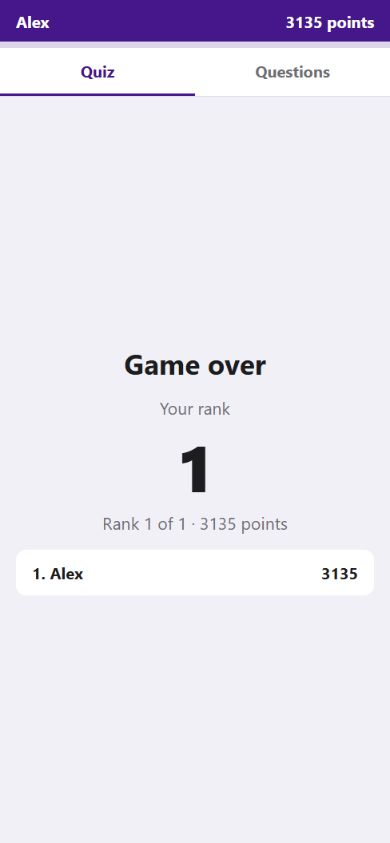
\includegraphics[width=49mm]{../images/manual/18-phone-final-rank.jpg}\par
{\manualcaption The phone displays the final rank at the end.\par}
\end{minipage}\hfill%
\begin{minipage}[t]{195mm}\vspace{0pt}
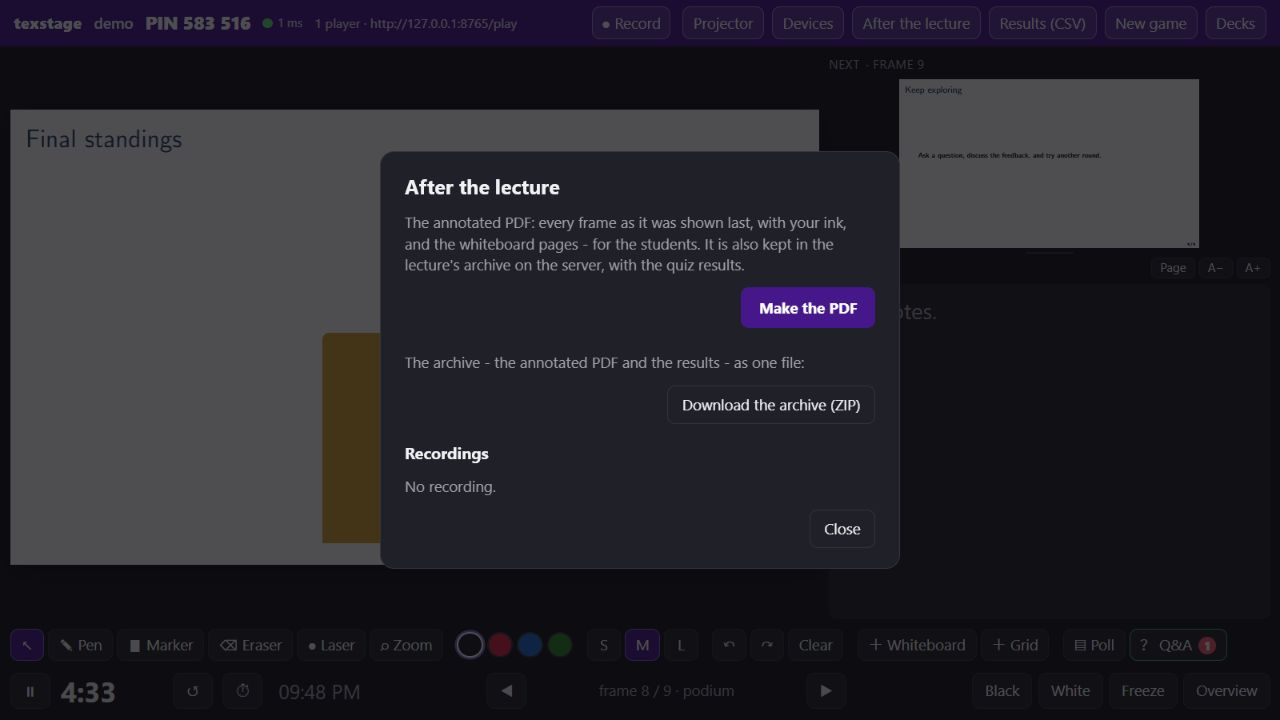
\includegraphics[width=\linewidth]{../images/manual/19-after-the-lecture.jpg}\par
{\manualcaption Generate the annotated PDF and download the archive. No recording was made in this example.\par}
\end{minipage}\par\medskip
A podium slide finishes the quiz session and shows final standings on phones. \textbf{After the lecture} opens the export tools; opening that panel alone does not end a quiz. \textbf{New game}, or returning to the join slide after a podium, starts a new session with a new PIN.\par

Choose \textbf{Make the PDF} for the last-shown version of each frame, ink and whiteboard pages; the PDF is also saved to the server archive. \textbf{Results (CSV)} exports participant results. The archive ZIP combines the annotated PDF, if generated, and results. Recorded takes appear in the Recordings list. Review student-facing files before sharing; keep result data and presenter credentials private.\par


% Author a small quiz and choose the right export
\manualsection{Author a small quiz and choose the right export}
A quiz belongs in a Beamer document. Give each question a stable, unique ID. Mark correct choices with \texttt{\textbackslash{}choice*}; ordinary \texttt{\textbackslash{}choice} entries are distractors. \texttt{\textbackslash{}explain} supplies feedback. The existing authoring guide describes all question types and options.\par

\begin{Verbatim}
\documentclass{beamer}
\usepackage{texquiz}
\begin{document}
\quizjoinframe
\begin{quiz}[id=planet, time=20]{Which planet is known as the Red Planet?}
  \choice{Venus}
  \choice*{Mars}
  \explain{Mars appears reddish because of iron oxide on its surface.}
\end{quiz}
\quizpodiumframe
\end{document}
\end{Verbatim}

{\small
\begin{tabular}{>{\raggedright\arraybackslash}p{\dimexpr0.380000\linewidth-2\tabcolsep\relax}>{\raggedright\arraybackslash}p{\dimexpr0.620000\linewidth-2\tabcolsep\relax}}
\rowcolor{manualPurple}
\color{white}\bfseries Command or file & \color{white}\bfseries Use \\
texstage pdf deck.tex & Handout with quiz placeholders; the default PDF mode. \\
\rowcolor{manualPale}
texstage pdf --solutions deck.tex & Questions with correct answers and explanations. \\
texstage pdf --present deck.tex & A static PDF preview of the live presentation steps. \\
\rowcolor{manualPale}
texstage build deck.tex & Build the live PowerPoint file, static PowerPoint fallback and server bundle. \\
deck.bundle.zip & Upload this package to a texstage server. \\
\rowcolor{manualPale}
deck.pptx / deck-static.pptx & The live deck needs the server/add-in and may carry its presenter key. The static fallback has no live quiz. \\
\end{tabular}}\par\medskip

Output normally goes to \texttt{texquiz-out} beside the source; use \texttt{--output-dir} to choose another location. For PowerPoint, install the add-in on the presenting PC, then use \texttt{texstage present deck.tex --powerpoint}. Rehearse with \texttt{texstage check deck.pptx} and start from its preparation slide. Keep the live PPTX out of student downloads.\par


% Troubleshoot before and during a session
\manualsection{Troubleshoot before and during a session}
{\small
\begin{tabular}{>{\raggedright\arraybackslash}p{\dimexpr0.250000\linewidth-2\tabcolsep\relax}>{\raggedright\arraybackslash}p{\dimexpr0.750000\linewidth-2\tabcolsep\relax}}
\rowcolor{manualPurple}
\color{white}\bfseries Symptom & \color{white}\bfseries What to do \\
A phone cannot open the join page & Use the actual reachable server address, not localhost or 127.0.0.1. Check the network and firewall. Open /api/status at that same address from the phone. Campus networks may isolate devices; use a suitable hotspot or configured hosted server/tunnel. \\
\rowcolor{manualPale}
The PIN is rejected & Read the current PIN from the presenter or join slide. New game creates a different PIN; an old screenshot or previous session PIN will not work. \\
The phone has no answer buttons & A lobby or reading screen is normal. Wait for the presenter to open the round. If it says Paused, the presenter must resume the quiz. \\
\rowcolor{manualPale}
The phone says Reconnecting & Restore its network connection and keep the same browser/tab. A saved participant token lets the same player resume after a reload. A different browser or cleared storage can lose that identity. \\
The presenter needs a key & Use the correct server's authorized presenter key or pair the device from the laptop. Participants need only the PIN and nickname. \\
\rowcolor{manualPale}
Projector does not open or move & Allow its pop-up for this server. Move the window manually if automatic placement is unavailable. Use extended displays so the presenter stays private. \\
The projector seems stuck & Check Freeze, Black and White. Return to normal display. Also check the presenter connection indicator. \\
\rowcolor{manualPale}
A question will not restart & Going backwards preserves its state. Choose Ask again for practice or New game for a new session; review the rewind effects first. \\
A deck or stage PDF is missing & Reload the library after building, upload the .bundle.zip to the intended server, or rebuild without --no-stage. Check the first LaTeX error if the build failed. \\
\rowcolor{manualPale}
Recording has no sound & Check browser permission, the selected microphone and its level meter. Make a short rehearsal recording and play it back. \\
\end{tabular}}\par\medskip

Before class: verify the build, join from a real phone, rehearse one question and its reveal, check the projector and notes, and know which static PDF/PPTX you will use if the live connection fails.\par


% Participant quick reference
\manualsection{Participant quick reference}
\manualsubheading{Join}
\begin{itemize}
\item Scan the QR code or open the address shown in the room.
\item Enter the current PIN and a nickname. Tap Join and wait for You're in!.
\item Keep the same browser tab open so a reconnection can restore your place.
\end{itemize}

\manualsubheading{Answer}
\begin{itemize}
\item Read the question first. The presenter decides when answers open.
\item Single choice or true/false: tap one answer; it submits immediately.
\item Multiple choice: select all intended answers, then tap Submit.
\item Number, text, ordering or sketch: complete the input, then tap Submit.
\item Wait for Answer sent and then the reveal. Your result and score appear when the round allows it.
\end{itemize}

\manualsubheading{Ask for help}
\begin{itemize}
\item If Questions is available, submit a question there or upvote another question.
\item If you cannot connect, tell the presenter. Check the current PIN and that your network can reach the displayed address.
\item Do not enter a presenter key. The participant page needs only the session PIN and nickname.
\end{itemize}


% Presenter shortcut card
\manualsection{Presenter shortcut card}
{\small
\begin{tabular}{>{\raggedright\arraybackslash}p{\dimexpr0.240000\linewidth-2\tabcolsep\relax}>{\raggedright\arraybackslash}p{\dimexpr0.280000\linewidth-2\tabcolsep\relax}>{\raggedright\arraybackslash}p{\dimexpr0.250000\linewidth-2\tabcolsep\relax}>{\raggedright\arraybackslash}p{\dimexpr0.230000\linewidth-2\tabcolsep\relax}}
\rowcolor{manualPurple}
\color{white}\bfseries Action & \color{white}\bfseries Shortcut & \color{white}\bfseries Action & \color{white}\bfseries Shortcut \\
Next / previous & Right / Left, PageDown / PageUp & Overview & G \\
\rowcolor{manualPale}
Jump to frame & Number, then Enter & Black / White & B / W \\
Freeze / unfreeze & F & Elapsed timer & T \\
\rowcolor{manualPale}
Pen / Marker / Eraser & P / H / E & Laser / Zoom & L / Z \\
Whiteboard / Grid & N / Shift+N & Undo / Redo & Ctrl+Z / Ctrl+Y \\
\end{tabular}}\par\medskip

This shortcut card is for the texstage browser presenter. PowerPoint uses its own presentation controls. The lecture timer shortcut does not pause a quiz countdown.\par


% About the screenshots and further help
\manualsection{About the screenshots and further help}
The screenshots show texstage 0.2.1.dev0 from the release-preparation source revision \texttt{daf0976b67954613a839b111f9696e41ab000433}, captured on 27 October 2026. The desktop viewport was 1280 x 720; phone screens used a 390 x 844 browser viewport. Browser size is emulated; physical phone hardware was not tested for these captures.\par

All content, nicknames and results are synthetic. Alex is an example participant. The PIN, local address and scores are illustrations, not credentials for a running class. The demonstration server was isolated from existing courses and presenter data. Phone controls shown here are in English; the participant interface can use German according to browser language.\par

The source deck is \href{../../examples/manual/demo.tex}{examples/manual/demo.tex}. It uses 240-second quiz rounds for capture and rehearsal. Replace the example local join address and choose a realistic round duration for teaching. Live session join information comes from the server's advertised address.\par

{\small
\begin{tabular}{>{\raggedright\arraybackslash}p{\dimexpr0.250000\linewidth-2\tabcolsep\relax}>{\raggedright\arraybackslash}p{\dimexpr0.750000\linewidth-2\tabcolsep\relax}}
\rowcolor{manualPurple}
\color{white}\bfseries Companion guide & \color{white}\bfseries Contents \\
installation.md & Source/wheel installation, TeX requirements, hosting overview and common setup failures. \\
\rowcolor{manualPale}
authoring.md & Full quiz syntax, question options, presentation workflows and hosting details. \\
integration.md & Supported Python integration API for companion course tools. \\
\rowcolor{manualPale}
dependencies.md & Locked environments and dependency updates. \\
SECURITY.md & Private reporting and handling of keys, inputs and server data. \\
\rowcolor{manualPale}
releasing.md & Publication prerequisites and candidate validation. \\
\end{tabular}}\par\medskip

For a reproducible problem, record the package version, operating system, browser, TeX version and exact command, and reduce it to a synthetic example. Remove presenter keys and participant data from logs or screenshots before sharing them.\par

Screenshot sources and hashes are listed in \href{../images/manual/captures.json}{images/manual/captures.json}. The \href{../manual-maintenance.md}{manual maintenance guide} explains how to refresh the images and regenerate all reading formats.\par


% LaTeX reference: packages and loading
\manualsection{LaTeX reference: packages and loading}
This reference covers all four shipped LaTeX packages and their author-facing commands, environments, keys and theme hooks. Beamer, TikZ and other upstream commands retain their own upstream contracts. Core developer interfaces are identified separately. Examples target the current 0.2.1.dev0 candidate.\par

{\small
\begin{tabular}{>{\raggedright\arraybackslash}p{\dimexpr0.350000\linewidth-2\tabcolsep\relax}>{\raggedright\arraybackslash}p{\dimexpr0.650000\linewidth-2\tabcolsep\relax}}
\rowcolor{manualPurple}
\color{white}\bfseries Syntax / option & \color{white}\bfseries Meaning and default \\
\texttt{texstage.sty} & Shared mode selection, page records, geometry and phone assets. Loaded automatically by every content package; it does not select a course theme. \\
\rowcolor{manualPale}
\texttt{texquiz.sty} & Quizzes, quiz/answer frame options, join/leaderboard/podium frames and customizable answer rendering. Requires the core, TikZ and pdftexcmds; QR support is optional. \\
\texttt{texvideo.sty} & The video command, static posters and live playback metadata. Requires the core, graphicx and TikZ; qrcode is optional. \\
\rowcolor{manualPale}
\texttt{texactivity.sty} & Tuple and code activities, prompts, seeds and reference answers. Requires the core and Beamer facilities. \\
\texttt{docs/manual-latex/manual.sty} & Documentation layout only: headings, typography, tables and page furniture. Do not load it in a lecture deck. \\
\end{tabular}}\par\medskip

\begin{Verbatim}
\documentclass[aspectratio=169]{beamer}
\usepackage{texquiz}
\usepackage{texvideo}     % only needed for video
\usepackage{texactivity}  % only needed for activities
\begin{document}
% Frames and quiz environments go here.
\end{document}
\end{Verbatim}

The texstage CLI supplies the installed style directory. For plain pdfLaTeX, put the four generic files on the TeX search path or use the repository-relative loading shown in the reference example. Do not mix package copies from different revisions. DBIS themes and course notation belong to lecture-tools.\par


% Build modes and notes
\manualsection{Build modes and notes}
{\small
\begin{tabular}{>{\raggedright\arraybackslash}p{\dimexpr0.350000\linewidth-2\tabcolsep\relax}>{\raggedright\arraybackslash}p{\dimexpr0.650000\linewidth-2\tabcolsep\relax}}
\rowcolor{manualPurple}
\color{white}\bfseries Syntax / option & \color{white}\bfseries Meaning and default \\
\texttt{\textbackslash{}def\textbackslash{}texstagemode\{handout\}} & Define before documentclass. Quiz and answer frames become neutral placeholders; videos remain posters and activities retain their prompts. \\
\rowcolor{manualPale}
\texttt{\textbackslash{}def\textbackslash{}texstagemode\{solutions\}} & Questions, correct choices and explanations are visible. Activity references are printed. Videos remain posters. \\
\texttt{\textbackslash{}def\textbackslash{}texstagemode\{present\}} & Live layout and .tqz metadata. The builder makes the browser bundle and PowerPoint exports; compiling a raw PDF does not start a live session. \\
\rowcolor{manualPale}
\texttt{\textbackslash{}def\textbackslash{}texquizmode\{...\}} & Legacy alias accepted when texstagemode is absent. An explicitly defined texstagemode takes precedence. \\
\texttt{No explicit mode} & At begin-document, Beamer notes enabled selects solutions; otherwise handout. Use explicit modes when this distinction matters. \\
\rowcolor{manualPale}
\texttt{\textbackslash{}texquiznotes} & Build-owned switch: empty selects extraction-oriented notes on the right; stage selects separate note pages, omits extra phone-asset pages and stabilizes the stage PDF. Let the CLI set it. \\
\end{tabular}}\par\medskip

\begin{Verbatim}
texstage pdf examples/reference/reference.tex
texstage pdf --solutions examples/reference/reference.tex
texstage pdf --present examples/reference/reference.tex
texstage build examples/reference/reference.tex
\end{Verbatim}

The core needs a LaTeX kernel dated 2023-06-01 or newer. Present mode supports pdfLaTeX and has a LuaLaTeX code path; the supplied examples are validated with pdfLaTeX. XeLaTeX is rejected for present mode. Live video codecs, external display placement and Office playback need separate platform rehearsal.\par


% Quiz environments and body commands
\manualsection{Quiz environments and body commands}
{\small
\begin{tabular}{>{\raggedright\arraybackslash}p{\dimexpr0.350000\linewidth-2\tabcolsep\relax}>{\raggedright\arraybackslash}p{\dimexpr0.650000\linewidth-2\tabcolsep\relax}}
\rowcolor{manualPurple}
\color{white}\bfseries Syntax / option & \color{white}\bfseries Meaning and default \\
\texttt{\textbackslash{}begin\{quiz\}[keys]\{question\} ... \textbackslash{}end\{quiz\}} & Between frames, creates its own frame. Inside a frame, that frame must have the quiz option. The question is required; one quiz per frame, no authored overlays in quiz frames. \\
\rowcolor{manualPale}
\texttt{\textbackslash{}quizsetup\{keys\}} & Sets deck-wide defaults and display strings. Call after loading texquiz and after any theme whose defaults you want to override. \\
\texttt{\textbackslash{}choice[id=label]\{text\}} & Adds an incorrect choice. Nonempty text; id defaults to A, B, ... in authored order. Explicit ids use 1-32 ASCII letters/digits/hyphens and must be unique within the quiz. \\
\rowcolor{manualPale}
\texttt{\textbackslash{}choice*[id=label]\{text\}} & Marks a correct choice. Several starred choices infer multiple choice; explicit type=multiple also permits one starred choice. \\
\texttt{\textbackslash{}explain\{text\}} & At most one explanation per quiz. Shown on the built-in reveal/solutions page; with reveal=none, explain on a separate answer frame. \\
\rowcolor{manualPale}
\texttt{\textbackslash{}accept\{text\}} & One or more accepted answers for type=text. Hyperref converts the authored text to plain Unicode for scoring. Use texorpdfstring for unsupported math/macros. \\
\texttt{\textbackslash{}step\{text\}} & One nonempty ordering item, written in the correct order. The displayed order is shuffled. \\
\rowcolor{manualPale}
\texttt{\textbackslash{}note\{text\}, \textbackslash{}label\{name\}} & Beamer commands accepted in a quiz body; notes and stable slide references remain available. The quiz title is not its id. \\
\end{tabular}}\par\medskip

Choice, explanation, acceptance and step commands are local to the quiz body. Do not put arbitrary paragraphs, verbatim or listings directly in that body. Put supporting material in a surrounding fragile,quiz frame and keep the question/reveal layout compact. Explicit choice ids identify authored choices; the public A/B/... labels follow the displayed order after shuffling.\par


% Quiz types and scoring
\manualsection{Quiz types and scoring}
{\small
\begin{tabular}{>{\raggedright\arraybackslash}p{\dimexpr0.350000\linewidth-2\tabcolsep\relax}>{\raggedright\arraybackslash}p{\dimexpr0.650000\linewidth-2\tabcolsep\relax}}
\rowcolor{manualPurple}
\color{white}\bfseries Syntax / option & \color{white}\bfseries Meaning and default \\
\texttt{single} & 2-6 choices, exactly one correct. Inferred when one choice is starred. \\
\rowcolor{manualPale}
\texttt{multiple} & 2-6 choices, at least one correct. Exact-set scoring by default; partial=true enables partial credit. \\
\texttt{truefalse} & answer=true or answer=false; no choice commands. Labels come from true-label and false-label. \\
\rowcolor{manualPale}
\texttt{poll} & 2-6 unstarred choices. Explicit type=poll; select=single by default or multiple. No correct answer and no points. \\
\texttt{numeric} & Decimal answer and optional tolerance; no answer means an unscored estimate. Bounds may produce a slider. \\
\rowcolor{manualPale}
\texttt{text} & At least one accept command. Scoring normalizes case, accents and whitespace; author meaningful accepted variants rather than relying on literal TeX source. \\
\texttt{open} & Unscored free text. display=wordcloud by default, or list; max-chars defaults to 80. \\
\rowcolor{manualPale}
\texttt{order} & 2-6 step commands in correct order. Exact ordering by default; partial=true credits correctly placed items. \\
\texttt{sketch} & Unscored drawing input. No choices, accepted answers, steps or answer key; presenter chooses drawings for display. \\
\end{tabular}}\par\medskip

Type inference checks ordering items, accepted text, choices, then a boolean/numeric answer. Polls, open text, sketches and numeric estimates without an answer should declare their type. Poll/open/sketch/estimate questions force points=none; explicitly requesting scoring for them is an error. Scoring is server behavior, not a LaTeX calculation.\par


% Quiz options: identity, timing and layout
\manualsection{Quiz options: identity, timing and layout}
{\small
\begin{tabular}{>{\raggedright\arraybackslash}p{\dimexpr0.350000\linewidth-2\tabcolsep\relax}>{\raggedright\arraybackslash}p{\dimexpr0.650000\linewidth-2\tabcolsep\relax}}
\rowcolor{manualPurple}
\color{white}\bfseries Syntax / option & \color{white}\bfseries Meaning and default \\
\texttt{id} & Required, unique across the deck: 1-63 characters, starts with a lower-case letter or digit, then lower-case letters/digits/hyphens. \\
\rowcolor{manualPale}
\texttt{type} & single, multiple, truefalse, poll, numeric, text, open, order or sketch; otherwise inferred when unambiguous. \\
\texttt{time} & Integer 5-240 seconds. Inherits quizsetup; initial default 20. \\
\rowcolor{manualPale}
\texttt{points} & standard, double or none. Inherits quizsetup; initial default standard, except forced-unscored types. \\
\texttt{leaderboard} & true/false; bare key means true. Default follows setup and is false for unscored questions unless explicitly set. Automatic result pages do not increment the authored frame number. \\
\rowcolor{manualPale}
\texttt{shuffle} & true/false; bare key means true. Initially false. Deterministic choice shuffling is shared between slide and phones; ordering questions are always shuffled. \\
\texttt{reveal} & slide (default) creates the built-in reveal; none defers it to an answer frame. \\
\rowcolor{manualPale}
\texttt{title} & Title of a generated quiz frame; initially Quiz. Inside an authored frame, use that frame title. A neutral title is used for handout placeholders. \\
\texttt{cols} & 1-6 forces the choice columns. Unset uses measured fitting and the theme maximum (2 in the generic theme). \\
\rowcolor{manualPale}
\texttt{partial} & Boolean, false by default; bare key means true. Meaningful for multiple choice and ordering; it changes credit, not which answer is fully correct. \\
\end{tabular}}\par\medskip

Time, points, leaderboard, shuffle, reveal and title have setup-level counterparts. Per-question values override them. Other question keys listed on the next page are not accepted by quizsetup.\par


% Quiz options: answer data
\manualsection{Quiz options: answer data}
{\small
\begin{tabular}{>{\raggedright\arraybackslash}p{\dimexpr0.350000\linewidth-2\tabcolsep\relax}>{\raggedright\arraybackslash}p{\dimexpr0.650000\linewidth-2\tabcolsep\relax}}
\rowcolor{manualPurple}
\color{white}\bfseries Syntax / option & \color{white}\bfseries Meaning and default \\
\texttt{select} & Only polls: single (default) or multiple. \\
\rowcolor{manualPale}
\texttt{answer} & true/false for truefalse; a decimal for numeric. Omit for an unscored numeric estimate. \\
\texttt{tolerance} & Numeric tolerance, default 0. Must be nonnegative. \\
\rowcolor{manualPale}
\texttt{min, max} & Optional numeric bounds. min must not exceed max; a scored answer interval must intersect the allowed range. Both bounds select a phone slider. \\
\texttt{step} & Positive numeric slider increment, default 1 when a slider is used. At least one value min + k*step must fall in the correct interval. \\
\rowcolor{manualPale}
\texttt{unit} & Optional numeric unit text, initially empty, e.g. ms. \\
\texttt{display} & Only open text: wordcloud (default) or list. \\
\rowcolor{manualPale}
\texttt{max-chars} & Open-text input limit, default 80; the build validates 1-200. The TeX parser accepts digits before the bundle validation applies the range. \\
\end{tabular}}\par\medskip

\begin{Verbatim}
\begin{quiz}[id=latency, type=numeric, answer=2.5,
    tolerance=0.1, min=0, max=5, step=0.1, unit={ms}]{Latency?}
  \explain{The measured latency was 2.5 ms.}
\end{quiz}
\begin{quiz}[id=term, type=text]{Name the language.}
  \accept{SPARQL}
  \accept{\texorpdfstring{\textsc{sparql}}{SPARQL}}
\end{quiz}
\end{Verbatim}

Use ordinary decimal notation such as -1.5, not exponents or a comma decimal separator. Avoid irrelevant keys: the supported contract is the type-specific one above, even where a parser accepts an unused value.\par


% Setup defaults and session frames
\manualsection{Setup defaults and session frames}
{\small
\begin{tabular}{>{\raggedright\arraybackslash}p{\dimexpr0.350000\linewidth-2\tabcolsep\relax}>{\raggedright\arraybackslash}p{\dimexpr0.650000\linewidth-2\tabcolsep\relax}}
\rowcolor{manualPurple}
\color{white}\bfseries Syntax / option & \color{white}\bfseries Meaning and default \\
\texttt{\textbackslash{}quizsetup\{time=20, points=standard\}} & Initial time and scoring defaults; same valid values as quiz options. \\
\rowcolor{manualPale}
\texttt{leaderboard=true, shuffle=false, reveal=slide} & Initial global behavior. A DBIS theme changes some of these defaults. \\
\texttt{title=Quiz, join-url=\{\}} & Default quiz title; no static join address until you supply one. The live server supplies the active address/PIN. \\
\rowcolor{manualPale}
\texttt{\textbackslash{}quizjoinframe[title=..., note=\{...\}]} & Creates a join frame outside any frame. Default title Join the quiz. Static modes show join-text and join-url; live mode displays the active session. \\
\texttt{\textbackslash{}quizleaderboardframe[title=..., note=\{...\}]} & Explicit standings frame outside any frame. Default title Leaderboard. This is separate from automatically inserted post-question standings. \\
\rowcolor{manualPale}
\texttt{\textbackslash{}quizpodiumframe[title=..., note=\{...\}]} & Final standings outside any frame. Default title Final standings; reaching it finishes the live quiz session. \\
\texttt{title, note (frame keys)} & The only keys accepted by these three frame commands. note is optional, may contain paragraphs, and is carried to presenter notes. \\
\rowcolor{manualPale}
\texttt{\textbackslash{}begin\{frame\}[quiz]} & Hosts an inline quiz. The whole frame is replaced by a neutral placeholder in handout mode. Use fragile,quiz when the supporting material contains listings. \\
\texttt{\textbackslash{}begin\{frame\}[answer=quiz-id]} & Reveals that quiz on this frame. With bare answer the frame is hidden in the handout, but has no quiz-id association. \\
\end{tabular}}\par\medskip

For delayed answers, give the quiz reveal=none, then write an answer=its-id frame later. Do not put quizjoinframe, quizleaderboardframe or quizpodiumframe inside a frame: each command creates one.\par


% Quiz display strings (1/2)
\manualsection{Quiz display strings (1/2)}
These quizsetup keys replace visible static slide text. Values below are the generic English defaults, before a course theme is loaded. They do not configure the language of the phone application.\par

{\small
\begin{tabular}{>{\raggedright\arraybackslash}p{\dimexpr0.350000\linewidth-2\tabcolsep\relax}>{\raggedright\arraybackslash}p{\dimexpr0.650000\linewidth-2\tabcolsep\relax}}
\rowcolor{manualPurple}
\color{white}\bfseries Setup key & \color{white}\bfseries Initial text \\
\texttt{join-title} & Join the quiz \\
\rowcolor{manualPale}
\texttt{join-text} & During the lecture, join with your phone using the PIN shown on this slide. \\
\texttt{leaderboard-title} & Leaderboard \\
\rowcolor{manualPale}
\texttt{podium-title} & Final standings \\
\texttt{handout-heading} & Live quiz \\
\rowcolor{manualPale}
\texttt{handout-text} & This question is asked live in the lecture. \\
\texttt{results-text} & The results are shown live in the lecture. \\
\rowcolor{manualPale}
\texttt{answer-title} & Answer \\
\texttt{answer-heading} & Answer \\
\rowcolor{manualPale}
\texttt{answer-text} & The answer is shown in the lecture. \\
\end{tabular}}\par\medskip

\begin{Verbatim}
\quizsetup{title=Question, true-label=Yes, false-label=No}
\end{Verbatim}

Use braces for values containing commas or paragraphs. Change the setup after loading a theme to retain your override. For the DBIS German strings and its leaderboard defaults, see the separate lecture-tools style reference.\par


% Quiz display strings (2/2)
\manualsection{Quiz display strings (2/2)}
These quizsetup keys replace visible static slide text. Values below are the generic English defaults, before a course theme is loaded. They do not configure the language of the phone application.\par

{\small
\begin{tabular}{>{\raggedright\arraybackslash}p{\dimexpr0.350000\linewidth-2\tabcolsep\relax}>{\raggedright\arraybackslash}p{\dimexpr0.650000\linewidth-2\tabcolsep\relax}}
\rowcolor{manualPurple}
\color{white}\bfseries Setup key & \color{white}\bfseries Initial text \\
\texttt{true-label} & True \\
\rowcolor{manualPale}
\texttt{false-label} & False \\
\texttt{number-hint} & Enter a number on your phone. \\
\rowcolor{manualPale}
\texttt{text-hint} & Type your answer on the phone. \\
\texttt{multiple-hint} & Several answers can be correct. \\
\rowcolor{manualPale}
\texttt{poll-hint} & Tick all that apply. \\
\texttt{order-hint} & Put the items in the right order on your phone. \\
\rowcolor{manualPale}
\texttt{sketch-hint} & Draw your answer on your phone. \\
\texttt{answer-label} & Answer: \\
\rowcolor{manualPale}
\texttt{accepted-label} & Accepted answers: \\
\end{tabular}}\par\medskip

\begin{Verbatim}
\quizsetup{title=Question, true-label=Yes, false-label=No}
\end{Verbatim}

Use braces for values containing commas or paragraphs. Change the setup after loading a theme to retain your override. For the DBIS German strings and its leaderboard defaults, see the separate lecture-tools style reference.\par


% Quiz theme hooks
\manualsection{Quiz theme hooks}
{\small
\begin{tabular}{>{\raggedright\arraybackslash}p{\dimexpr0.350000\linewidth-2\tabcolsep\relax}>{\raggedright\arraybackslash}p{\dimexpr0.650000\linewidth-2\tabcolsep\relax}}
\rowcolor{manualPurple}
\color{white}\bfseries Syntax / option & \color{white}\bfseries Meaning and default \\
\texttt{\textbackslash{}texquizprompt\{text\}} & Draws the question within its supplied width. Generic default: large text. \\
\rowcolor{manualPale}
\texttt{\textbackslash{}texquizchoice \{label\} \{shape\} \{width\} \{height\} \{state\} \{content\}} & Draw an answer with exactly the supplied geometry. height may be empty for natural height. Reference point must be the lower-left corner. \\
\texttt{\textbackslash{}texquizchoicefont} & Answer font, generic default normalsize. Redefine with renewcommand. \\
\rowcolor{manualPale}
\texttt{\textbackslash{}texquizchoiceoverhead} & Width reserved besides answer text, generic default 2.31cm. Must match the actual box padding and live-count reserve. \\
\texttt{\textbackslash{}texquizmaxcols} & Maximum automatically chosen columns, generic default 2. \\
\rowcolor{manualPale}
\texttt{\textbackslash{}texquizexplanation\{text\}} & Reveal/solutions explanation; default is a light panel. \\
\texttt{\textbackslash{}texquizhint\{text\}} & Input hint; generic default small text in texquiz-hint color. \\
\rowcolor{manualPale}
\texttt{\textbackslash{}texquizbadge\{n\}} & Inline shape badge, n=1..6: triangle, diamond, circle, square, star, hexagon. \\
\end{tabular}}\par\medskip

The choice label is A, B, ... or an ordering rank. shape is 1-6; state is plain, correct or wrong. Correct and wrong choices must look identical in state plain. Keep geometry consistent because the server overlays counts and live content on the recorded rectangles.\par

Colors are texquiz-1 through texquiz-6, texquiz-correct, texquiz-panel and texquiz-hint. They style the PDF/deck rendering; a TeX color change alone does not restyle the phone UI. Private macros containing @ or \_\_ are implementation details.\par

\begin{Verbatim}
\renewcommand{\texquizprompt}[1]{{\Large\bfseries #1\par}}
\end{Verbatim}


% Video command and options
\manualsection{Video command and options}
Load texvideo, then place the command inside a Beamer frame. Every video requires a local JPEG/PNG poster. Paths are relative to the deck directory. The poster determines the rendered aspect ratio; match it to the video.\par

{\small
\begin{tabular}{>{\raggedright\arraybackslash}p{\dimexpr0.350000\linewidth-2\tabcolsep\relax}>{\raggedright\arraybackslash}p{\dimexpr0.650000\linewidth-2\tabcolsep\relax}}
\rowcolor{manualPurple}
\color{white}\bfseries Syntax / option & \color{white}\bfseries Meaning and default \\
\texttt{\textbackslash{}video[keys]\{source\}} & source is a local media file or online address. A local file must exist. The command can be used in overlays and repeated frames. \\
\rowcolor{manualPale}
\texttt{poster} & Required image. The bundle builder accepts .jpg, .jpeg and .png. \\
\texttt{width, height} & Optional graphicx dimensions; with neither, the poster uses its natural dimensions. Supply one dimension to preserve aspect ratio. \\
\rowcolor{manualPale}
\texttt{id} & Optional; derived from source basename/address when omitted, lower-cased and normalized. Use an explicit stable id for predictable reuse. \\
\texttt{start, end} & Optional times in seconds. Omitted means the player default beginning/end. Supply nonnegative values with end after start. Playback interpretation is player-specific. \\
\rowcolor{manualPale}
\texttt{loop, muted, autoplay} & Booleans, initially false; a bare key means true. autoplay requests playback on entering the slide, subject to browser policies. \\
\texttt{url} & Optional online copy for the handout link/QR. If omitted for an online video, its source URL is used; a local video otherwise shows its filename. \\
\end{tabular}}\par\medskip

\begin{Verbatim}
\begin{frame}{A short demonstration}
  \video[id=demo-clip, poster=poster.jpg, width=.75\textwidth,
         start=5, end=20, muted]{clip.mp4}
\end{frame}
\end{Verbatim}

Reusing an id retains the same video and playback state. Its source, poster and playback keys must agree. Repeating the same id twice on one slide is an error. Give separate videos distinct ids.\par


% Video output and portability
\manualsection{Video output and portability}
{\small
\begin{tabular}{>{\raggedright\arraybackslash}p{\dimexpr0.350000\linewidth-2\tabcolsep\relax}>{\raggedright\arraybackslash}p{\dimexpr0.650000\linewidth-2\tabcolsep\relax}}
\rowcolor{manualPurple}
\color{white}\bfseries Syntax / option & \color{white}\bfseries Meaning and default \\
\texttt{Handout / solutions} & Poster plus a play mark and filename or link. A QR code is added for an online link when qrcode.sty is available. The PDF does not embed a playing video. \\
\rowcolor{manualPale}
\texttt{Browser presentation} & Local media is copied into the bundle. YouTube, Vimeo and supported direct media URLs get live players; an unsupported online URL produces a warning and keeps its poster. \\
\texttt{PowerPoint, live and static} & Local media becomes a native movie object. An online video becomes a linked poster. Browser-only playback options are not applied by the current native PowerPoint movie writer. \\
\rowcolor{manualPale}
\texttt{Local formats} & The builder recognizes .mp4, .m4v, .webm and .mov. MP4 with H.264/AAC is the documented cross-workflow target; actual playback depends on installed/browser codecs. \\
\texttt{Network and size} & Online playback needs its provider/network. Local media is duplicated into the bundle and both PPTX files; videos over 100 MiB cause a build warning. \\
\end{tabular}}\par\medskip

Compilation checks poster geometry and packaging, not successful playback on every browser or Office version. Rehearse actual media on the presentation device. The documentation example uses a synthetic external URL so it builds without downloading media; it is explicitly a poster/link example, not a playable movie test.\par

The full command contract is in texvideo.sty and src/texstage/build/video.py. Do not interpret a warning-only online URL as proof that an embedded browser player exists for it.\par


% Activity environment and common options
\manualsection{Activity environment and common options}
{\small
\begin{tabular}{>{\raggedright\arraybackslash}p{\dimexpr0.350000\linewidth-2\tabcolsep\relax}>{\raggedright\arraybackslash}p{\dimexpr0.650000\linewidth-2\tabcolsep\relax}}
\rowcolor{manualPurple}
\color{white}\bfseries Syntax / option & \color{white}\bfseries Meaning and default \\
\texttt{\textbackslash{}begin\{activity\}[keys] ... \textbackslash{}end\{activity\}} & Place inside a Beamer frame; one activity per frame. The environment does not create a frame. A repeated frame may reuse the same unchanged activity id. \\
\rowcolor{manualPale}
\texttt{\textbackslash{}prompt\{formatted text\}} & Activity instruction. Used in the static box and rendered for phones. One prompt per activity is the supported authoring pattern. \\
\texttt{\textbackslash{}reference\{verbatim text\}} & Code activity reference answer; may be repeated for alternative solutions. Use a fragile frame for inline verbatim. File form: reference=answer.rq or an engine-appropriate text file. \\
\rowcolor{manualPale}
\texttt{\textbackslash{}seed\{verbatim text\}} & Inline code-activity data. Use a fragile frame, or prefer seed=data.ttl / seed=data.sql. If a seed file and inline seed are both supplied, the file takes precedence. \\
\texttt{id} & Required, 1-63 lower-case letters/digits/hyphens, starting with a letter or digit. Same id must keep the same definition. \\
\rowcolor{manualPale}
\texttt{input} & tuple (default) or code. Code input requires engine and seed data. \\
\texttt{width, height} & Default linewidth and 0.6 textheight. Size the box to leave room for the frame title and other material. \\
\rowcolor{manualPale}
\texttt{open} & auto (default) opens when the frame is reached; manual waits for the presenter. \\
\texttt{limit} & Contributions per student: 1-50. Default 10 for tuple, 5 for code. \\
\end{tabular}}\par\medskip

The exported TexactivityPrompt, TexactivityReference and TexactivitySeed commands are the implementation backing for the local prompt/reference/seed aliases. Use the local names inside activity. Arbitrary body text is not a substitute for prompt.\par


% Tuple activities: options and example
\manualsection{Tuple activities: options and example}
{\small
\begin{tabular}{>{\raggedright\arraybackslash}p{\dimexpr0.350000\linewidth-2\tabcolsep\relax}>{\raggedright\arraybackslash}p{\dimexpr0.650000\linewidth-2\tabcolsep\relax}}
\rowcolor{manualPurple}
\color{white}\bfseries Syntax / option & \color{white}\bfseries Meaning and default \\
\texttt{fields} & Two or three labels. Default Subject, Predicate, Object. First/last fields become nodes; a third, middle field labels the edge. \\
\rowcolor{manualPale}
\texttt{suggest} & Optional comma-separated suggestions. At most 40 entries, each 1-60 characters, after conversion/unescaping. \\
\texttt{min} & Required supporting contributions before a tuple appears on the projector: integer 1-1000, default 1. \\
\rowcolor{manualPale}
\texttt{review} & Boolean, default false; bare key means true. Enables presenter review. \\
\texttt{terms} & exact (default) preserves term identity; loose groups case, accents and spacing. Use exact for RDF-like identifiers. \\
\rowcolor{manualPale}
\texttt{engine} & Not allowed for tuple input. Code-specific seed, reference and tokens produce build warnings if supplied to a tuple activity. \\
\end{tabular}}\par\medskip

\begin{Verbatim}
\begin{frame}{Build a small graph}
  \begin{activity}[id=class-graph, fields={Person, Knows, Person},
      suggest={Alice,Bob,Chris}, min=1, review, height=.5\textheight]
    \prompt{Add one connection between two people.}
  \end{activity}
\end{frame}
\end{Verbatim}

Handout, solutions and PowerPoint show the static activity prompt. Live interaction is implemented in the texstage browser presenter and phones. The current PowerPoint add-in implements quizzes, not live activities.\par


% Code activities: engines and data
\manualsection{Code activities: engines and data}
{\small
\begin{tabular}{>{\raggedright\arraybackslash}p{\dimexpr0.350000\linewidth-2\tabcolsep\relax}>{\raggedright\arraybackslash}p{\dimexpr0.650000\linewidth-2\tabcolsep\relax}}
\rowcolor{manualPurple}
\color{white}\bfseries Syntax / option & \color{white}\bfseries Meaning and default \\
\texttt{engine=sparql} & Queries a Turtle seed (.ttl). References contain SPARQL queries. \\
\rowcolor{manualPale}
\texttt{engine=sql} & Queries tables initialized by SQL statements (.sql), using the bundled SQLite browser engine. References contain SQL queries. \\
\texttt{engine=turtle} & Participants write Turtle. A .ttl seed supplies base/prefix declarations; seed triples are not copied into the participant graph. References contain Turtle graphs. \\
\rowcolor{manualPale}
\texttt{seed} & Required for code input, as a file or inline seed. UTF-8 text; a BOM is accepted for files. Maximum encoded seed size is 2 MiB. \\
\texttt{reference} & Optional reference file. Its text is appended to any inline references. Each reference is 1-2000 characters. References are private bundle answer data, not public phone seed data. \\
\rowcolor{manualPale}
\texttt{tokens} & Extra keyboard buttons: up to 40 entries of 1-60 characters. Engine punctuation is added automatically. Escape TeX punctuation in key values, e.g. backslash followed by \# or \%. \\
\texttt{Unused tuple keys} & fields, suggest, min, review and terms have no code-input effect and cause warnings when non-default values are supplied. \\
\end{tabular}}\par\medskip

The seed is distributed with the activity and is visible to participants; it must contain synthetic/public teaching data. A code activity can omit references for an exploratory task. Providing a reference is what permits comparison with a model result; it does not make arbitrary code input safe to run outside the supported browser engines.\par

The builder validates data sizes and engine-specific seed extensions. A plain PDF compile cannot establish that SQL/SPARQL/Turtle semantics or results match the teaching objective.\par


% Code activity example and build checks
\manualsection{Code activity example and build checks}
\begin{Verbatim}
\begin{frame}[fragile]{Query the people table}
  \begin{activity}[id=names, input=code, engine=sql,
      height=.4\textheight, open=manual, tokens={SELECT,FROM,ORDER BY}]
    \prompt{Return all names in alphabetical order.}
    \seed{CREATE TABLE people(name TEXT);
INSERT INTO people VALUES ('Bob'), ('Alice');}
    \reference{SELECT name FROM people ORDER BY name;}
  \end{activity}
\end{frame}
\end{Verbatim}

For ordinary course files, prefer seed=people.sql and reference=names.sql. This avoids embedding verbatim in a macro argument or a non-fragile frame. All paths are resolved from the deck directory; keep referenced files with the source export.\par

{\small
\begin{tabular}{>{\raggedright\arraybackslash}p{\dimexpr0.350000\linewidth-2\tabcolsep\relax}>{\raggedright\arraybackslash}p{\dimexpr0.650000\linewidth-2\tabcolsep\relax}}
\rowcolor{manualPurple}
\color{white}\bfseries Syntax / option & \color{white}\bfseries Meaning and default \\
\texttt{texstage pdf --solutions} & Shows activity references and quiz answers. Verify that long code and explanations fit the frame. \\
\rowcolor{manualPale}
\texttt{texstage build} & Validates the .tqz records, seed files, media and public/private bundle split. It also checks quiz layout in present and solutions modes. \\
\texttt{Browser rehearsal} & Open one activity, submit synthetic input, inspect results and reveal behavior. Compilation alone is not a browser/Office interoperability test. \\
\end{tabular}}\par\medskip

Runnable examples and an isolated validation command are provided in \href{../../examples/reference/README.md}{examples/reference/README.md}. They use dedicated output/data directories and do not load existing courses.\par


% Activity labels and documentation helpers
\manualsection{Activity labels and documentation helpers}
The activity label hooks are ordinary macros. Redefine them after loading texactivity to localize static slide text; they do not change the phone UI language.\par

{\small
\begin{tabular}{>{\raggedright\arraybackslash}p{\dimexpr0.420000\linewidth-2\tabcolsep\relax}>{\raggedright\arraybackslash}p{\dimexpr0.580000\linewidth-2\tabcolsep\relax}}
\rowcolor{manualPurple}
\color{white}\bfseries Hook & \color{white}\bfseries Default and contract \\
\texttt{\textbackslash{}texactivitylabel} & No arguments. Default: Live activity -- on your phones. \\
\rowcolor{manualPale}
\texttt{\textbackslash{}texactivityreferencelabel} & No arguments. Default: Reference. Used above solution reference text. \\
\end{tabular}}\par\medskip

\begin{Verbatim}
\renewcommand{\texactivitylabel}{Live task -- use your phone}
\end{Verbatim}

\texttt{docs/manual-latex/manual.sty} only controls this manual: landscape A4, typography, colors, tables and headers/footers. Its \texttt{\textbackslash{}manualsection\{title\}} starts a new page/section; \texttt{\textbackslash{}manualsubheading\{title\}} formats a small heading; \texttt{\textbackslash{}manualcaption} selects caption text. The document supplies \texttt{\textbackslash{}manualversion} and \texttt{\textbackslash{}manualdate}.\par

This documentation style loads fontenc, lmodern, geometry, xcolor, graphicx, array, fancyhdr, fancyvrb, enumitem, titlesec, hyperref, bookmark, microtype and upquote. Compile the documentation with pdfLaTeX; its PDF text mapping uses pdfTeX commands. It is not a lecture-deck package.\par


% Core interfaces for package developers
\manualsection{Core interfaces for package developers}
These expl3 interfaces are shared by texquiz, texvideo and texactivity. They are documented for maintainers of the current candidate, not a promise of a versioned plugin ABI. Use ExplSyntaxOn when writing extension code; ordinary slide authors should use the content packages.\par

{\small
\begin{tabular}{>{\raggedright\arraybackslash}p{\dimexpr0.350000\linewidth-2\tabcolsep\relax}>{\raggedright\arraybackslash}p{\dimexpr0.650000\linewidth-2\tabcolsep\relax}}
\rowcolor{manualPurple}
\color{white}\bfseries Syntax / option & \color{white}\bfseries Meaning and default \\
\texttt{\textbackslash{}texstage\_if\_mode:nTF \{mode\}\{yes\}\{no\}} & Tests the resolved mode; T and F variants are also defined. \\
\rowcolor{manualPale}
\texttt{\textbackslash{}texstage\_error:n \{message\}} & Raises a package error. \\
\texttt{\textbackslash{}texstage\_hex:n \{text\}} & Encodes record text as hex. V and e variants accept a variable or expanded content. \\
\rowcolor{manualPale}
\texttt{\textbackslash{}texstage\_emit:n \{record\}} & Writes an expanded record immediately in present mode. \\
\texttt{\textbackslash{}texstage\_on\_page:n \{record\}} & Writes at shipout, freezing the current logical page number; position values are expanded later. \\
\rowcolor{manualPale}
\texttt{\textbackslash{}texstage\_page\_record:nnn \{kind\}\{id\}\{phase\}} & Associates a live item and phase with a page. \\
\texttt{\textbackslash{}texstage\_savepos:, \textbackslash{}texstage\_lastx:, \textbackslash{}texstage\_lasty:} & Save the current position and read engine coordinates in scaled points. \\
\rowcolor{manualPale}
\texttt{\textbackslash{}texstage\_rect:nnnnn \{id\}\{phase\}\{key\}\{width\}\{height\}} & Records a rectangle at the current lower-left reference point. \\
\texttt{\textbackslash{}texstage\_vmark:nnn \{id\}\{phase\}\{key\}} & Records a horizontal boundary across linewidth in vertical mode for a live region. \\
\end{tabular}}\par\medskip

Do not emit arbitrary records from a course deck. The Python build registry must understand the content type, its public metadata, private answer data, phone assets and rendering. Shipout and shrink corrections are coordinated by the core.\par


% Core asset and layout helpers
\manualsection{Core asset and layout helpers}
{\small
\begin{tabular}{>{\raggedright\arraybackslash}p{\dimexpr0.350000\linewidth-2\tabcolsep\relax}>{\raggedright\arraybackslash}p{\dimexpr0.650000\linewidth-2\tabcolsep\relax}}
\rowcolor{manualPurple}
\color{white}\bfseries Syntax / option & \color{white}\bfseries Meaning and default \\
\texttt{\textbackslash{}texstage\_check\_mark:nn \{kind\}\{id\}} & Adds a layout-check log mark outside handout mode. \\
\rowcolor{manualPale}
\texttt{\textbackslash{}texstage\_stage\_notes:} & Enables stage-note bookkeeping and deterministic pdfTeX metadata; normally called through the build-owned notes switch. \\
\texttt{\textbackslash{}texstage\_asset\_box:nn \{width\}\{content\}} & Typesets the next extra-page asset into a global box. \\
\rowcolor{manualPale}
\texttt{\textbackslash{}texstage\_asset\_add:nnn \{id\}\{key\}\{natural width\}} & Associates that box with an item and records its unbroken natural width. Call after asset\_box. \\
\texttt{\textbackslash{}texstage\_asset:nnnn \{id\}\{key\}\{width\}\{content\}} & Combined asset creation and natural-width measurement. \\
\rowcolor{manualPale}
\texttt{\textbackslash{}texstage\_ship\_assets:} & Ships recorded extra pages after the slides. The normal stage compile suppresses these; authors should not call it themselves. \\
\texttt{\textbackslash{}texstage\_vfill:} & Vertical fill that wins over Beamer top-aligned-frame fill. \\
\rowcolor{manualPale}
\texttt{\textbackslash{}texstage\_vbox\_set:Nnn \{box variable\}\{width\}\{content\}} & Sets a zero-depth box whose reference point is its lower-left corner. \\
\texttt{\textbackslash{}texstage\_once:n \{code\}} & Runs code only on the first overlay of the current frame. \\
\rowcolor{manualPale}
\texttt{\textbackslash{}texstage\_check\_outside\_frame:n \{command name\}} & Errors when a frame-creating command is used inside a frame. \\
\end{tabular}}\par\medskip

Names containing @, names beginning \_\_, parser temporaries and global state variables are implementation details. The core also patches Beamer shrink/shipout handling; do not copy those internals into themes. The maintained inventory records source hashes so changes require a documentation review.\par


% LaTeX examples and common authoring failures
\manualsection{LaTeX examples and common authoring failures}
{\small
\begin{tabular}{>{\raggedright\arraybackslash}p{\dimexpr0.350000\linewidth-2\tabcolsep\relax}>{\raggedright\arraybackslash}p{\dimexpr0.650000\linewidth-2\tabcolsep\relax}}
\rowcolor{manualPurple}
\color{white}\bfseries Syntax / option & \color{white}\bfseries Meaning and default \\
\texttt{Unknown key or invalid id} & Check the correct key namespace: quizsetup, quiz, choice, special frame, video or activity. Use stable ids and avoid underscores in quiz/activity ids. \\
\rowcolor{manualPale}
\texttt{Text outside a quiz command} & Move material into the surrounding quiz frame, or into the question/choice/explanation argument. \\
\texttt{Reference/seed breaks compilation} & Use a fragile frame for inline verbatim, or external UTF-8 data/reference files. \\
\rowcolor{manualPale}
\texttt{No correct slider value} & Choose bounds and a positive step that actually contain a value in answer +/- tolerance. \\
\texttt{Answers appear in a handout} & Check the selected build mode and whether authored answer frames carry the answer option. \\
\rowcolor{manualPale}
\texttt{Static activity in PowerPoint} & Expected for this candidate. Use the browser presenter for live activities. \\
\texttt{Overfull or excessive shrink} & Shorten the content, reduce material on the frame, or select appropriate columns/box sizes. Run the checked build rather than hiding the warning. \\
\rowcolor{manualPale}
\texttt{Theme overlay is misaligned} & Keep answer-box width/height and lower-left reference point consistent with the hook contract. \\
\end{tabular}}\par\medskip

The compiled reference example covers every quiz type, delayed answers, explicit session frames, video poster packaging and tuple/code activity records. Coverage is an inventory of the documented project interfaces; it does not claim to document all commands provided by LaTeX, Beamer, TikZ or other dependencies.\par

The \href{../latex-reference-inventory.json}{reference inventory} and \href{../../examples/reference/README.md}{example build instructions} accompany this chapter. Existing courses and pinned styles do not need to change to read or build these isolated examples.\par

\end{document}
